\documentclass[12pt,a4paper,oneside,openany]{book}
\usepackage{graphicx}
\usepackage{amsmath}
\usepackage{amssymb}
\usepackage{empheq}
\usepackage{physics}
\usepackage{subcaption}
\usepackage{braket} % Per la notazione di Dirac
\usepackage{verbatim} % Per commentare più righe alla volta
\usepackage{circuitikz} % Per il generatore DC nello sputtering
\usepackage{float} % Per il comando [H]
\usepackage{tikz} % Per i disegni
\usepackage{changepage} % Per rendere le figure più larghe del testo
\usepackage[backend=biber,style=numeric,citestyle=numeric]{biblatex} % Per la bibliografia
\addbibresource{Bibliography.bib} % Importo il file con la bibliografia


\usepackage{fancyhdr}
\pagestyle{fancy}

\setlength{\headheight}{15pt}

\fancyhf{} % pulisce tutto

% intestazioni (valide per tutte le pagine)
\fancyhead[L]{\nouppercase{\rightmark}} % titolo capitolo a sinistra
\fancyhead[R]{\thepage}                 % numero pagina a destra

% linea sotto l’intestazione
\renewcommand{\headrulewidth}{0.4pt}

% evita corsivo e maiuscole forzate
\renewcommand{\chaptermark}[1]{\markboth{#1}{}}
\renewcommand{\sectionmark}[1]{\markright{#1}}


\newcommand{\RomanNumeralCaps}[1] % Per i numeri romani
{\MakeUppercase{\romannumeral #1}}

\renewcommand\thesubfigure{\Roman{subfigure}} % numeri romani maiuscoli nell'immagine

%\renewcommand\thesubfigure{\arabic{subfigure}} % numeri invece di lettere


\begin{document}
	\begin{titlepage}
	\centering
	
\includegraphics[width=0.7\textwidth]{Immagini/unipv_logo_new.jpg}\par\vspace{0.5cm}
	%		{\scshape\huge Universit\`a degli Studi di Pavia\par}
	%		\vspace{0.5cm}
	{\LARGE Dipartimento di Fisica\par
		\vspace{0.2cm}
		\Large\textit{Corso di laurea in Fisica}\par}
	\vspace{0.5cm}
	\rule{14cm}{0.1pt}
	
	\vspace{1.5cm}
	{\large\bfseries Superconductivity-Induced Shift in Resonant Field in a Superconductor-Ferromagnet-Superconductor Trilayer \par}
	\vspace{1.5cm}
	
	\vfill\large\begin{flushleft} Relazione per la laurea di:\\ \textbf{Leonardo Novello} % Text prior to the author name - right aligned and bold
	\end{flushleft}
	\vspace{.5cm}
	\begin{flushright}
		Supervisor:\\
		%https://accademiadellacrusca.it/it/consulenza/la-supervisora-supervisiona-non-supervede/27366
		\textbf{Prof. Giacomo Prando}\\[.3cm] % Advisor's/supervisor's name
		Cosupervisor:\\
		\textbf{Prof. Chiara Ciccarelli}\\[.3cm] % Advisor's/supervisor's name
	\end{flushright}
	
	
	
	\vfill
	
	% Bottom of the page
	{\large Anno accademico 2024 -- 2025\par}
\end{titlepage}

\newpage

\begin{comment}
	\clearpage
	\thispagestyle{empty} % niente intestazioni o numero di pagina
	\vspace*{\fill}
	
	%\begin{flushright}
	\noindent \emph{There is no such thing as a painless lesson, they just don't exist. Sacrifices are necessary. You can’t gain anything without losing something first. Although if you can endure that pain and walk away from it, you’ll find that you now have a heart strong enough to overcome any obstacle. Yeah, a heart made Fullmetal!}\\[1em]
	Edward Elric
	%\end{flushright}
	
	\vspace*{\fill}
	\clearpage    
\end{comment}

\begin{comment}
	\clearpage
	\thispagestyle{empty} % niente intestazioni o numero di pagina
	\vspace*{\fill}
	
	%\begin{flushright}
	\begin{figure}[H]
		\centering
		
\includegraphics[width=\linewidth]{immagini/onepiecepeoplesdreams.jpg}
	\end{figure}
	%\end{flushright}
	
	\vspace*{\fill}
	\clearpage    
\end{comment}

\tableofcontents

\chapter{Introduction}
Ferromagnetism and superconductivity were long considered incompatible due to their opposite ordering. However, when superconductors and ferromagnets are brought together, they give rise to a range of intriguing physical phenomena. In particular, the possibility of influencing the magnetization of a ferromagnetic system through superconductivity opens promising perspectives for the development of new memory and spintronic devices.

This thesis presents an investigation of the magnetization dynamics in superconductor–ferromagnet–superconductor (S/F/S) thin-film multilayers, conducted during my summer internship at the Cavendish Laboratory in Cambridge under the supervision of Professor Chiara Ciccarelli. During this period, I had the opportunity to participate in several experiments conducted by her group aimed at understanding the origin of the change in magnetic anisotropy induced by the superconducting layers in these trilayer systems.

The second chapter introduces the theoretical concepts necessary to interpret the experimental results. These include the fundamental properties of ferromagnetic and superconducting materials and their proximity effects, the theory of ferromagnetic resonance (FMR), the experimental technique used to probe the samples, and a review of the existing literature reporting a superconductivity-induced shift in the resonant field, together with its proposed explanations.

The third chapter describes the experimental setup used to perform the measurements.

Finally, the fourth chapter presents the data collected during the experiments and discusses how they relate to the results reported in the literature and to the theoretical model under investigation.

\chapter{Theoretical Background}

\section{Ferromagnetism}
\subsection{Maxwell's equations in matter}

The time evolution of the electric field $\mathbf{E}$ and the magnetic flux density $\mathbf{B}$ is governed by Maxwell's equations:

\begin{empheq}[left=\empheqlbrace]{align}
	& \nabla \cdot \mathbf{E} = \frac{\rho}{\varepsilon_0} \label{eq:maxwell1} \\
	& \nabla \times \mathbf{E} = -\frac{\partial \mathbf{B}}{\partial t} \label{eq:maxwell2} \\
	& \nabla \cdot \mathbf{B} = 0 \label{eq:maxwell3} \\
	& \nabla \times \mathbf{B} = \mu_0 \mathbf{J} + \mu_0 \varepsilon_0 \frac{\partial \mathbf{E}}{\partial t} \label{eq:maxwell4}
\end{empheq}

\vspace{.3cm}
\noindent where $\rho$ is the electric charge density, $\mathbf{J}$ is the electric current density. These equations, together with the Lorentz force law,
\begin{align}
	\mathbf{F} = q \, (\mathbf{E} + \mathbf{v} \times \mathbf{B})
\end{align}
which gives the force acting on a particle of charge $q$ moving with velocity $\mathbf{v}$ in an electromagnetic field $(\mathbf{E}, \mathbf{B})$, constitute the theory of classical electrodynamics.  

From \ref{eq:maxwell3}, $\mathbf{B}$ can be written as the curl of a vector field $\mathbf{A}$ called the vector potential
\begin{align}
	\mathbf{B} = \boldsymbol{\nabla} \times \mathbf{A}
	\label{potenziale_vettore}
\end{align}
substituting \ref{potenziale_vettore} in \ref{eq:maxwell2} we get
\begin{align}
	\boldsymbol{\nabla} \times \bigg( \mathbf{E} + \dfrac{\partial \mathbf{A}}{\partial t} \bigg) = \mathbf{0}
\end{align}
which implies that $\mathbf{E} + \dfrac{\partial \mathbf{A}}{\partial t}$ can be written as the negative gradient of a scalar field $V$, called the scalar potential
\begin{align*}
	\mathbf{E} + \dfrac{\partial \mathbf{A}}{\partial t} = - \nabla V
\end{align*}
\begin{align}
	\mathbf{E} = - \nabla V - \dfrac{\partial \mathbf{A}}{\partial t}
\end{align}

The energy density of the electromagnetic field is given by
\begin{align}
	u = \dfrac{\varepsilon_0}{2} E^2 + \dfrac{1}{2 \mu_0} B^2 .
\end{align}
The derivation can be found in \cite{Griffiths}. Therefore, the total energy required to generate an electromagnetic field $(\mathbf{E}, \mathbf{B})$ from a configuration with no field is
\begin{align}
	W = \int u \, d^3\mathbf{r} = \int \bigg( \dfrac{\varepsilon_0}{2} E^2 + \dfrac{1}{2 \mu_0} B^2 \bigg) d^3\mathbf{r}
	\label{energia_EM}
\end{align}

When dealing with matter, it is useful to introduce the following macroscopic quantities:

\noindent the polarization vector, defined as the electric dipole moment per unit volume:
\begin{align}
	\mathbf{P} = \dfrac{d\mathbf{p}}{dV}
\end{align}
the magnetization vector, defined as the magnetic dipole moment per unit volume:
\begin{align}
	\mathbf{M} = \dfrac{d\mathbf{m}}{dV}
\end{align}
the electric displacement field:
\begin{align}
	\mathbf{D} = \varepsilon_0 \mathbf{E} + \mathbf{P}
\end{align}
the magnetic field:
\begin{align}
	\mathbf{H} = \dfrac{\mathbf{B}}{\mu_0} - \mathbf{M}
	\label{Campo_magnetico}
\end{align}

\noindent In the presence of polarization and magnetization, the charge and current densities can be expressed as
\begin{align}
	\rho = \rho_f + \rho_b
\end{align}
where $\rho_b = \nabla \cdot \mathbf{P}$ is the bound charge density due to polarization and $\rho_f$ is the free charge density due to macroscopic charges, and
\begin{align}
	\mathbf{J} = \mathbf{J}_f + \mathbf{J}_b + \mathbf{J}_p
\end{align}
where $\mathbf{J}_b = \nabla \times \mathbf{M}$ is the bound current density due to magnetization, $\mathbf{J}_p = \frac{\partial \mathbf{P}}{\partial t}$ is the polarization current, and $\mathbf{J}_f$ is the free current density due to macrospopic currents.  

Using these definitions, Maxwell's equations can be rewritten in the equivalent form:
\begin{empheq}[left=\empheqlbrace]{align}
	& \nabla \cdot \mathbf{D} = \rho_f \label{eq:maxwellmat1} \\
	& \nabla \times \mathbf{E} = -\frac{\partial \mathbf{B}}{\partial t} \label{eq:maxwellmat2} \\
	& \nabla \cdot \mathbf{B} = 0 \label{eq:maxwellmat3} \\
	& \nabla \times \mathbf{H} = \mathbf{J}_f + \frac{\partial \mathbf{D}}{\partial t} \label{eq:maxwellmat4}
\end{empheq}

\vspace{.3cm}

\noindent The electric and magnetic susceptibilities are defined as:
\begin{align}
	\chi_e = \dfrac{1}{\varepsilon_0} \dfrac{\partial \mathbf{P}}{\partial \mathbf{E}}
\end{align}
\begin{align}
	\chi_m = \dfrac{\partial \mathbf{M}}{\partial \mathbf{H}}
	\label{eq:suscettività_magnetica}
\end{align}
Since $\dfrac{\partial \mathbf{A}}{\partial \mathbf{B}}$ is a tensor such that 
\[
\bigg( \dfrac{\partial \mathbf{A}}{\partial \mathbf{B}}\bigg)_{ij} = \dfrac{\partial A_i}{\partial B_j},
\] 
$\chi_e$ and $\chi_m$ are in general tensors depending on position $\mathbf{r}$. If a material is homogeneous, they do not depend on $\mathbf{r}$; if it is isotropic, they reduce to scalar quantities. Materials with $\chi_m > 0$ are called paramagnets, while those with $\chi_m < 0$ are called diamagnets. Materials in which $\chi_e$ and $\chi_m$ do not depend ont he fields are called linear.

\subsection{Properties of ferromagnetic materials}
Ferromagnets are nonlinear magnetic materials that, unlike paramagnets, do not require external fields to sustain their magnetization. This behavior is caused by several interactions, the most important being the exchange interaction, which forces the electrons in the material to align their magnetic dipoles. In contrast, linear magnetic materials can often be treated as collections of non-interacting dipoles. The response of the magnetization $\mathbf{M}$ of a ferromagnetic material as a function of the external magnetic field $\mathbf{H}$ is shown in Fig. \ref{fig:Hysteresis}.

\begin{figure}[H]
	\centering
	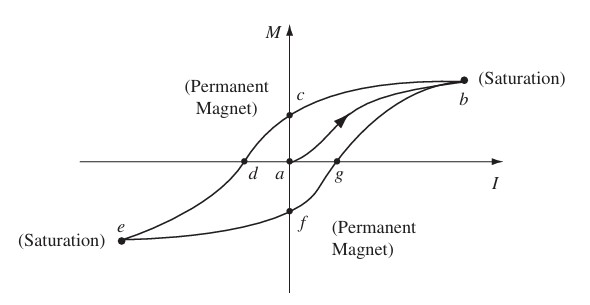
\includegraphics[width=\textwidth]{Immagini/Magnetism_images/Hysteresis.jpg}
	\caption{Magnetization $M$ of a ferromagnetic material as a function of the current $I$ flowing through a coil wrapped around the sample, which is proportional to the external magnetic field $H$.}
	\label{fig:Hysteresis}
\end{figure}

As $H$ is increased, the magnetization grows until it reaches its saturation value, corresponding to the state in which all magnetic dipoles are aligned. When the magnetic field is then reduced back to zero, the magnetization does not retrace the same path; instead, it retains a finite value known as the residual magnetization. If the magnetic field is increased and decreased in the opposite direction, the magnetization again saturates, eventually reaching the same magnitude with opposite sign. The closed path traced by the magnetization during this cycle is called the hysteresis loop.

This property, namely that the magnetization depends not only on the applied field but also on the history of the material, makes ferromagnets particularly useful for the development of magnetic memory devices.

As explained earlier, the behavior of ferromagnetic materials arises from different contributions to their total energy. The most important of these is the exchange interaction, a purely quantum-mechanical effect originating from the fact that electrons are indistinguishable fermions and therefore must have an antisymmetric total wavefunction. In the presence of electrostatic interactions, it can be shown (\cite{Carretta}) that two electrons minimize their energy when they occupy a triplet state with total spin $s=1$:
\begin{align*}
	\ket{1 \, 1} = \ket{\uparrow \, \uparrow}
\end{align*}
\begin{align*}
	\ket{1 \, 0} = \dfrac{1}{\sqrt{2}} (\ket{\uparrow \, \downarrow} + \ket{\downarrow \, \uparrow})
\end{align*}
\begin{align*}
	\ket{1 \, -1} = \ket{\downarrow \, \downarrow}
\end{align*}
This can be described with the effective hamiltonian:
\begin{align}
	H_{ex} = \sum_{i,j} -J_{i,j} \mathbf{S}_i \cdot \mathbf{S}_j
\end{align}
as explained in \cite{Blundell} the total exchange energy of a ferromagnetic material with continuosus magnetization can be written as:
\begin{align}
	E_{ex} = \dfrac{2JS^2z}{a} \int (\mathbf{\nabla} m_z) dV
\end{align}
where $a$ and $z$ are constants that depend on the crystal structure of the material and $\mathbf{m} = \frac{\mathbf{M}}{M_s}$. 

The Zeeman energy arises from the interaction between the magnetic moments and the external magnetic field and it is given by the equation:
\begin{align}
	E_z = - \mu_0 \int \mathbf{M} \cdot \mathbf{H} \, dV
\end{align}
Because $\mathbf{\nabla} \cdot \mathbf{H} = - \mathbf{\nabla} \cdot \mathbf{M}$ (it can be derived from equation \ref{Campo_magnetico}) then whenever $\mathbf{M}$ stops and starts, at the edges of a sample for example, the magnetic field diverges and this produces demagnetizing fields which fill space and which cost $\frac{B^2}{2 \mu_0}$ Joules of energy per cubic metre. The energy associated with the demagnetizing field is called demagnetization energy and it takes the value:
\begin{align}
	- \dfrac{\mu_0}{2} \int \mathbf{M} \cdot \mathbf{H_d} \, dV
\end{align}
where $\mathbf{H_d}$ is the demagnetizing field and the integral is taken over the volume of the sample. This interaction is responsible for the formation of magnetic domains in ferromagnetic materials. Finally, the anisotropy energy,arising from the spin–orbit interaction and the partial quenching of the orbital angular momentum, together with the shape anisotropy, which is the demagnetizing energy associated with the geometry of the sample, gives rise to magnetic anisotropy, meaning that ferromagnetic materials posses a magnetic easy axis, along which they are easy to magnetize, and a hard axis, along which they are harder to magnetize.

\subsection{Ferromagnetic resonance}
A system with angular momentum $\mathbf{L}$ and magnetic moment $\boldsymbol{\mu} = \gamma \mathbf{L}$ subject to an external magnetic field $\mathbf{H}$ evolves according to the following equation
\begin{align}
	\dfrac{d \mathbf{L}}{dt} = \boldsymbol{\mu} \times \mathbf{H}
\end{align}
The magnetization of a ferromagnetic sample is proportional to the sum of the magnetic moments of its electrons. Its dynamics is therefore expected to follow the equation
\begin{align}
	\dfrac{d \mathbf{M}}{dt} = \gamma \mathbf{M} \times \mathbf{H}
\end{align}
where $\mathbf{H}$ is the external applied magnetic field and $\gamma$ is the gyromagnetic ratio of an electron. However this form predicts perpetual precession without relaxation while experimentally, the magnetization is observed to align with the applied field after a finite time. To account for this, damping is introduced through the Gilbert term, which models a viscous-like relaxation. The full dynamics is described by the Landau–Lifshitz–Gilbert (LLG) equation
\begin{align}
	\dfrac{1}{\gamma}\dfrac{d \mathbf{M}}{dt} = \mathbf{M} \times \mathbf{H} + \dfrac{\alpha}{M_s} \left( \mathbf{M} \times \dfrac{d \mathbf{M}}{dt} \right)
	\label{eq:Landau_Lifshitz_Gilbert}
\end{align}
where $\alpha$ is the dimensionless Gilbert damping parameter and $M_s$ is the saturation magnetization.

Ferromagnetic resonance (FMR) is observed when a ferromagnetic material is subjected to both a constant (DC) magnetic field and a perpendicular oscillating (AC) magnetic field, typically at microwave frequencies. By linearizing and solving the Landau–Lifshitz–Gilbert (LLG) equation under these conditions, it can be shown that the power absorption profile of the system follows a Lorentzian line shape, which is characteristic of resonance phenomena. 

When an external magnetic field $\mathbf{H}$ is applied, the electronic energy levels split due to the Zeeman effect. Resonance occurs when the frequency of the transverse oscillating field matches the energy difference between Zeeman levels
\begin{align}
	\Delta E = g \mu_B B = h \nu
\end{align}
From the LLG equation, one can derive the relation between the resonance frequency $\omega_{res}$ and the resonance field $H_{res}$, known as the Kittel equation. Its form depends on the sample geometry and the orientation of the static field. For a thin film with an in-plane DC field, it reads
\begin{align}
	\omega_{res} = \gamma \sqrt{H_{res}(H_{res}+M_{eff})}
	\label{eq:Kittel}
\end{align}
The Gilbert damping can also be determined by measuring the linewidth of the resonance peak as a function of frequency via the relation
\begin{align}
	\Delta H = \Delta H_0 +\dfrac{2 \pi f \alpha}{\mu_0 \gamma}
\end{align}

\section{Superconductivity}
\subsection{Properties of Superconducting Materials}
The conductivity of a material is defined by the constitutive relation:
\begin{align}
	\mathbf{J} = \sigma \mathbf{E}
	\label{eq:Ohm}
\end{align}
Here $\mathbf{J}$ and $\mathbf{E}$ are, respectively, the electrical current density and the electric field at some point in the material.

The resistivity $\rho = \sigma^{-1} $ of most metals decreases as the temperature is lowered, eventually reaching a finite value determined by the presence of impurities. However there are some materials for which something different happens: when a superconducting material is cooled below a certain critical temperature $T_c$, its resisitiviy drops to zero. This is an example of a phase transition, which is a physical process where the properties of a macroscopic system change abruptly upon variation of a thermodynamic variable. Figure \ref{fig:ro_T} shows the difference in the temperature dependance of resistivity between a superconductor and a normal metal.
\begin{figure}[H]
	\centering
	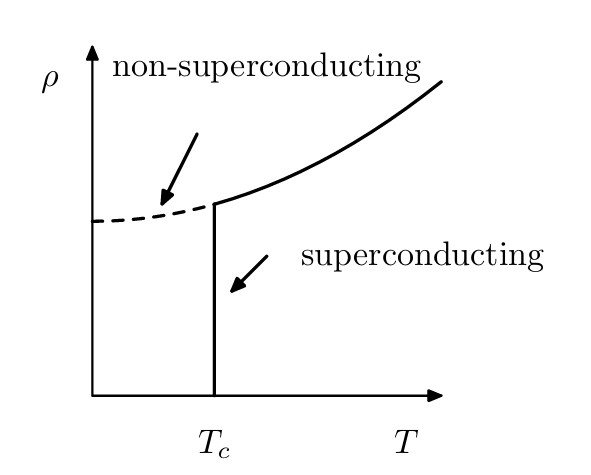
\includegraphics[width=0.6\linewidth]{Immagini/Superconductivity_images/Rho_vs_T_superconductor.jpg}
	\caption{Temperature dependence of the resistivity for a normal metal and a superconducting metal.}
	\label{fig:ro_T}
\end{figure}

Even though superconductors were historically discovered through the observation of zero resistivity, today this property is not regarded as the true definition of superconductivity. The fundamental proof that a material is superconducting is the demonstration of the Meissner effect, namely the complete expulsion of a weak external magnetic field. This is because the magnetic behavior of superconductors below their critical temperature cannot be fully explained by zero resistivity alone.  

As an example, let us consider a superconducting sample in the four configurations shown in Figure~\ref{fig:Meissner}.  

\begin{figure}[h]
	\centering
	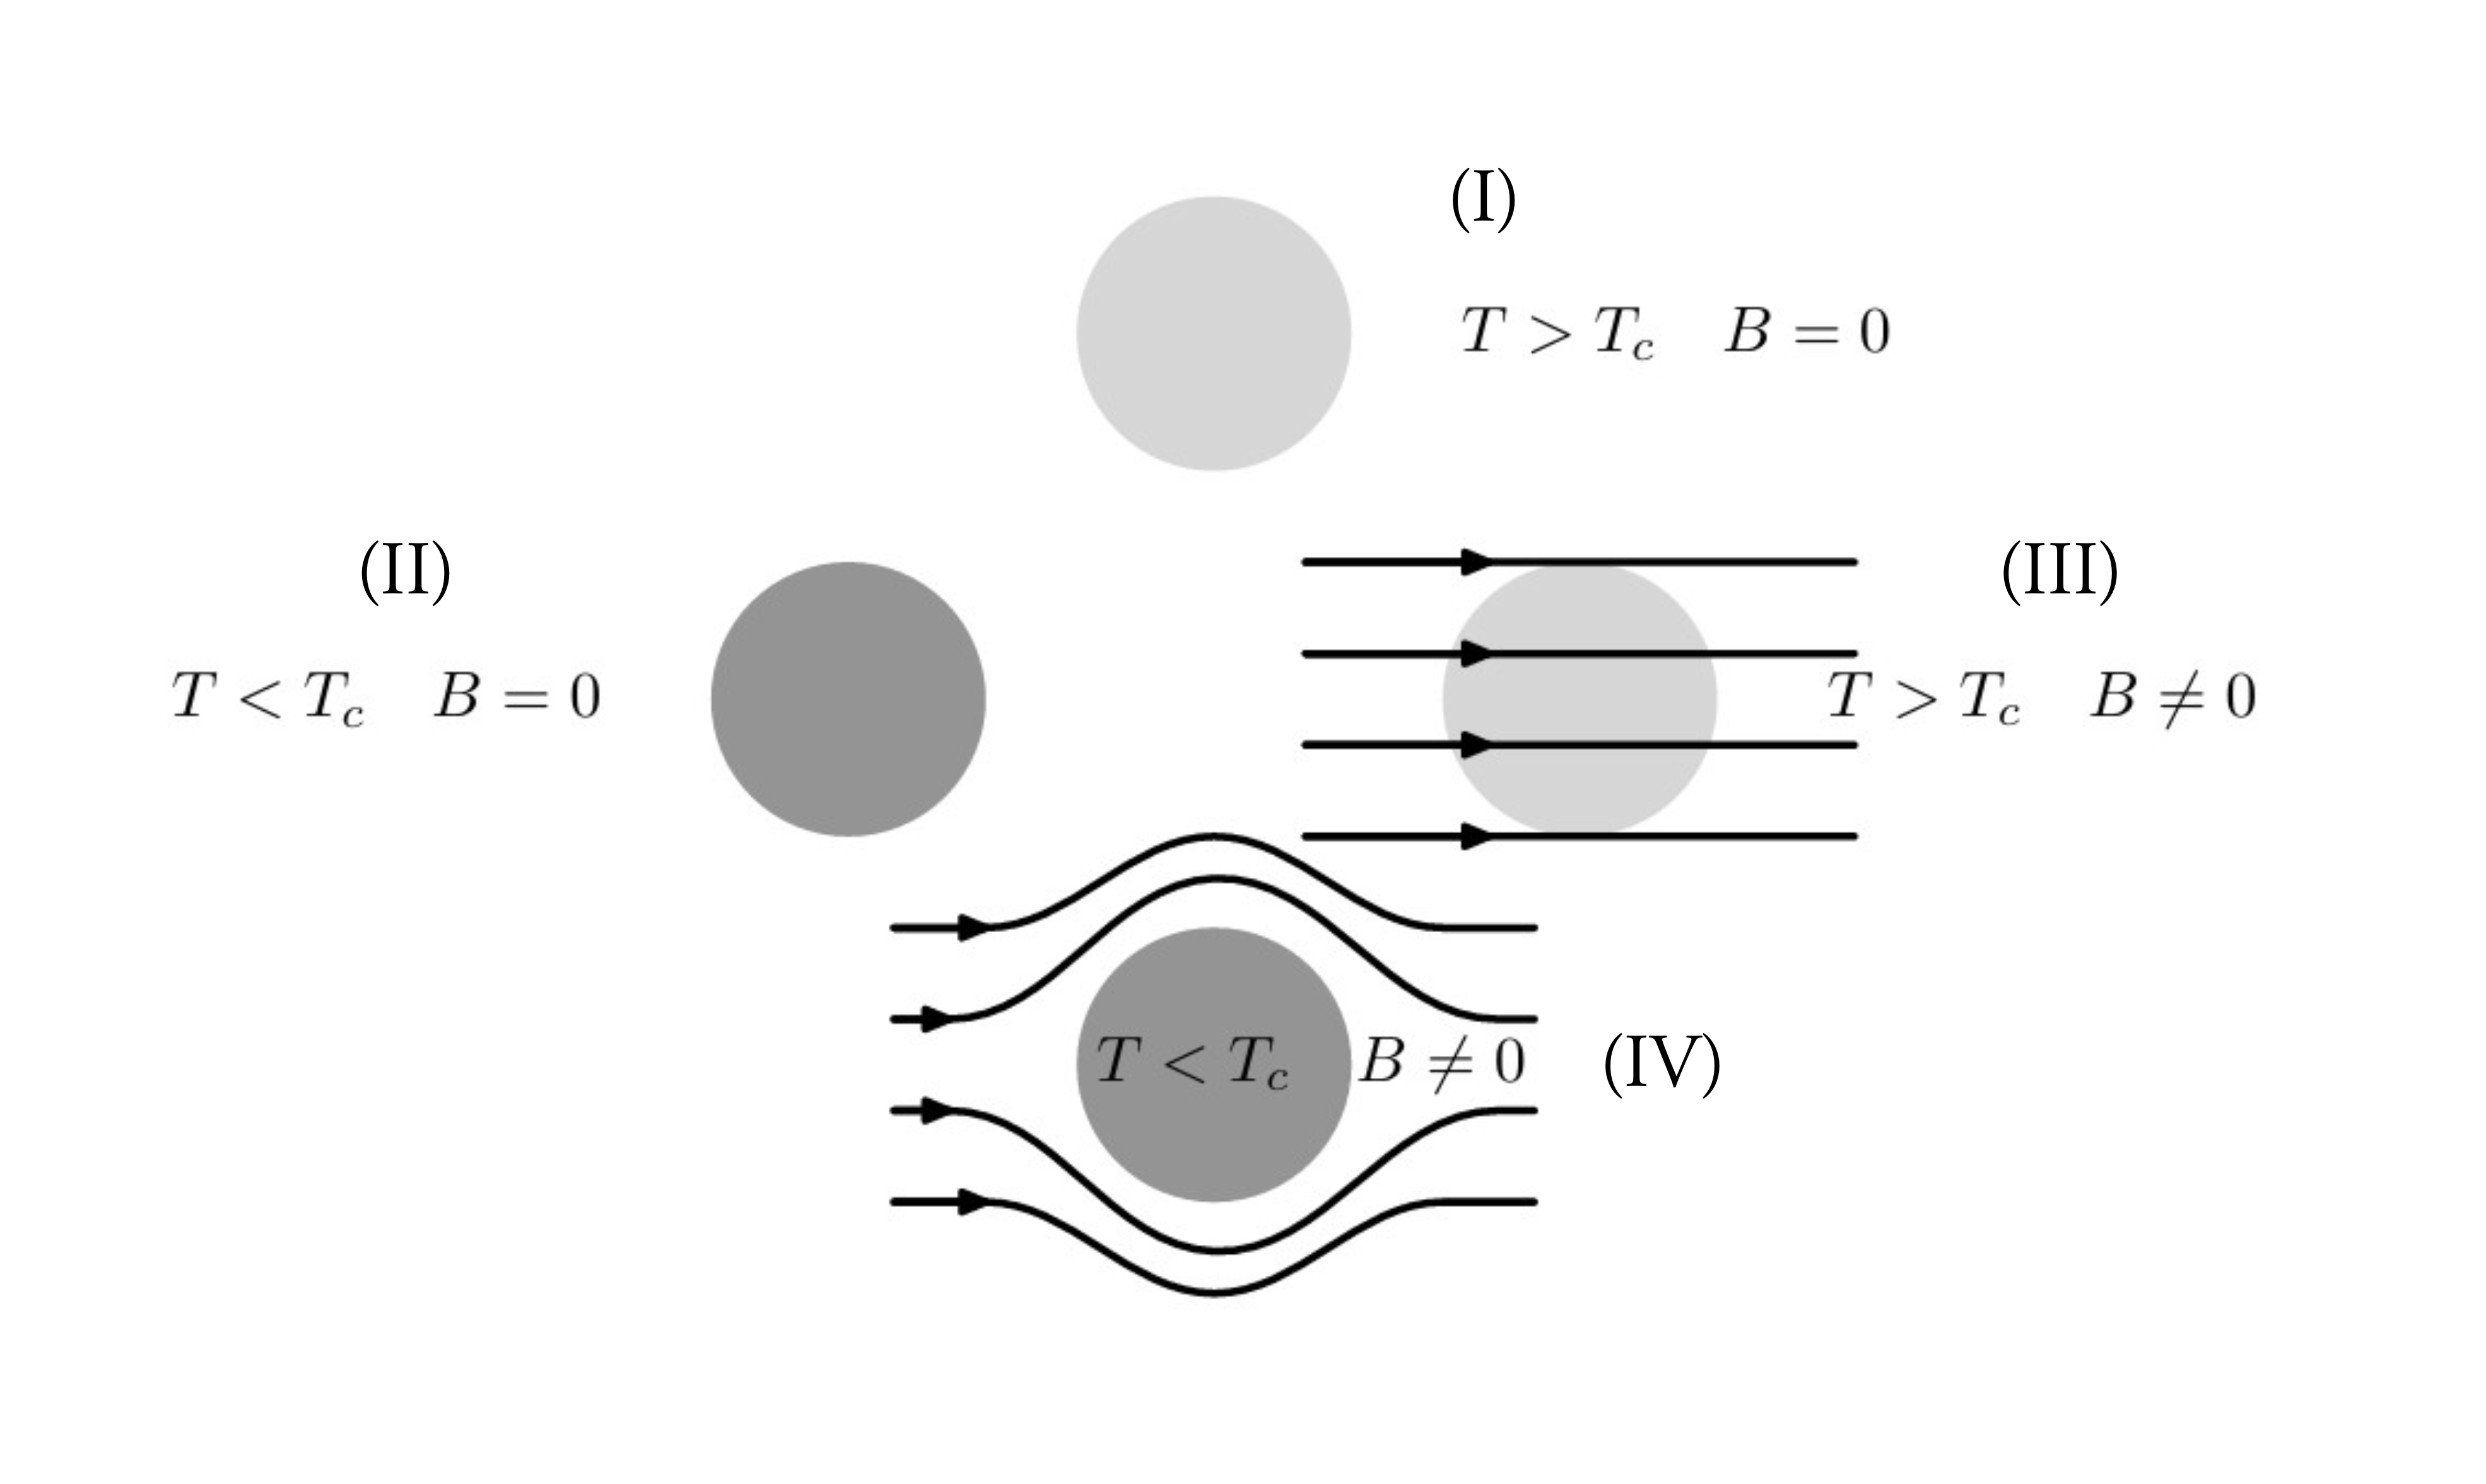
\includegraphics[width=\textwidth]{Immagini/Superconductivity_images/Meissner_5.png}
	\caption{}
	\label{fig:Meissner}
\end{figure}

\noindent Suppose initially the sample is in its normal state, $T > T_c$, and the external magnetic field is zero, as in (\RomanNumeralCaps{1}). If we cool the sample below $T_c$ while keeping the field zero, we obtain configuration (\RomanNumeralCaps{3}). Then, when the external field is gradually turned on, the field inside the sample must remain zero, as in (\RomanNumeralCaps{4}). This follows from the fact that with $\sigma = 0$ and a finite value of $\mathbf{J}$ in~\ref{eq:Ohm}, we must have
\begin{align}
	\mathbf{E} = \mathbf{0}
\end{align}
at every point inside the superconducting sample. Combining this with Maxwell’s equation~\ref{eq:maxwell2}, we obtain
\begin{align}
	\dfrac{\partial \mathbf{B}}{\partial t} = 0
\end{align}
throughout the superconductor. This implies that if the initial condition is $\mathbf{B} = \mathbf{0}$, it will remain so as long as the sample stays in the superconducting state, even when an external magnetic field is applied.  

If instead we start from (\RomanNumeralCaps{1}) and turn on the external magnetic field, the field will penetrate the sample as in (\RomanNumeralCaps{2}). However, if we then cool the sample below $T_c$ while maintaining the external field, we again obtain $\mathbf{B} = \mathbf{0}$ inside the superconductor, showing that the magnetic field is completely expelled. This behavior cannot be explained solely in terms of zero resistance. This is the difference between a superconductor and a perfect conductor: a perfect conductor is a material that preserves $\mathbf{B}$ no matter what its value is, a superconductor instead is a material that expels $\mathbf{B}$ so not only it cannot change but it has to be zero. 

The complete expulsion of the magnetic field means that, for weak magnetic fields, superconductors behave as perfect diamagnets. In fact, since $\mathbf{B} = \mathbf{0}$, from \ref{Campo_magnetico} we have
\begin{align}
	\mathbf{M} = - \mathbf{H},
	\label{eq:magnetizzazione_superconduttori}
\end{align}
and combining \ref{eq:magnetizzazione_superconduttori} with \ref{eq:suscettività_magnetica}, we find
\begin{align}
	\chi = \dfrac{\partial \mathbf{M}}{\partial \mathbf{H}} = -1.
\end{align}
The best way to detect superconductivity in some unknown sample is therefore to measure its susceptibility. If the sample is fully superconducting then $\chi_m$ as a function of $T$ will be something like the sketch in figure \ref{fig:Susceptibility_T}. Above $T_c$ it is a constant normal state value which is usually small and positive (paramagetic). Below $T_c$ one will find $\chi_m =-1$, evidence for the Meissner effect. This is usually considered much more reliable evidence for superconductivity in a sample than zero resistance alone would be.
\begin{figure}[H]
	\centering
	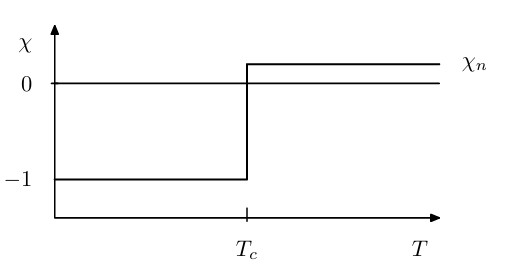
\includegraphics[width=0.7\textwidth]{Immagini/Superconductivity_images/Suscettivita_T.jpg}
	\caption{Magnetic susceptibility of a superconductor as a function of temperature.}
	\label{fig:Susceptibility_T}
\end{figure}
As the external field applied to a superconductor becomes stronger it turns out that either one of two possible things can happen.

For type \RomanNumeralCaps{1} superconductors, the $\mathbf{B}$ field remains zero inside the material until suddenly the superconductivity is destroyed. The field where this happens is called the critical field, $H_c$. The magnetization of a type \RomanNumeralCaps{1} obeys $\mathbf{M} = -\mathbf{H}$ for all fields less than $H_c$, and then becomes very close to zero for fields above $H_c$.

For type \RomanNumeralCaps{2} superconductors there are two different critical fields, denoted $H_{c1}$, the lower critical field, and $H_{c2}$ the upper critical field. For small values of applied field $\mathbf{H}$ the Meissner effect leads to $\mathbf{M} = -\mathbf{H}$ and there is no magnetic flux density inside the sample, $\mathbf{B} = \mathbf{0}$. However, once the field exceeds $H_{c1}$, magnetic flux does start to enter the superconductor and hence $\mathbf{B} = \mathbf{0}$, and $\mathbf{M}$ is closer to zero than the full Meissner value of $-\mathbf{H}$. Upon increasing the field H further the magnetic flux density gradually increases, until finally at $H_{c2}$ the superconductivity is destroyed and $\mathbf{M} \approx \mathbf{0}$. The phase below $H_{c1}$ is normally denoted the Meissner
state, while the phase between $H_{c1}$ and $H_{c2}$ is the Abrikosov or mixed state. 

The behaviour of the magnetization for type \RomanNumeralCaps{1} and type \RomanNumeralCaps{2} superconductors is sketched in figure \ref{Magnetizazzione_superconduttori}.
\begin{figure}[H]
	\centering
	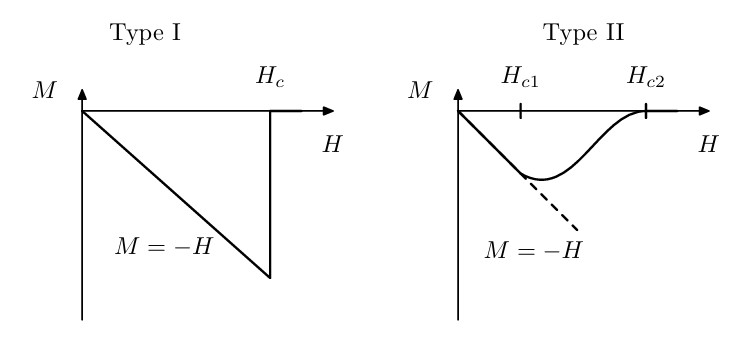
\includegraphics[width=0.9\linewidth]{Immagini/Superconductivity_images/M_H_1_vs_2.jpg}
	\caption{The magnetization as a function of the magnetic field in type \RomanNumeralCaps{1} and type \RomanNumeralCaps{2} superconductors.}
	\label{Magnetizazzione_superconduttori}
\end{figure}
As a function of the temperature the critical fields vary, and they all approach zero at the critical temperature $T_c$. The typical phase diagrams of type \RomanNumeralCaps{1} and type \RomanNumeralCaps{2} superconductors, as a function of $H$ and $T$ are shown in figure. 
\begin{figure}[H]
	\centering
	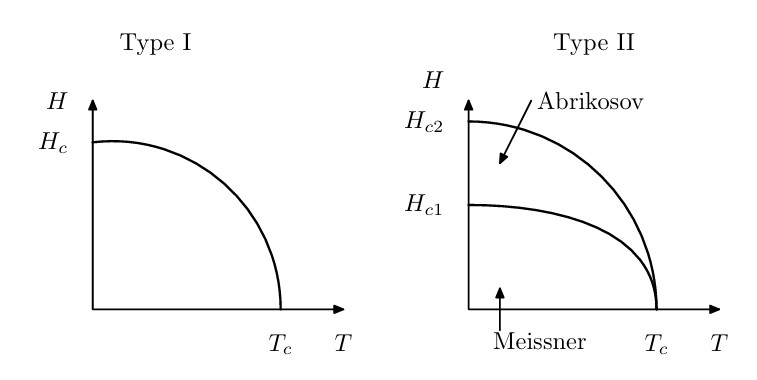
\includegraphics[width=0.9\linewidth]{Immagini/Superconductivity_images/Type_1_vs_2.jpg}
	\caption{The $H$-$T$ phase diagram of type \RomanNumeralCaps{1} and type \RomanNumeralCaps{2} superconductors.}
	\label{Diagramma_H_T_superconduttori}
\end{figure}

The physical reason for the thermodynamic phase between $H_{c1}$ and $H_{c2}$ is the presence of vortices: the magnetic field can enter the superconductor in the form of vortices, as shown in figure \ref{vortici}. Each vortex consists of a region of circulating supercurrent around a small central core which has essentially become normal metal. The magnetic field is able to pass through the sample inside the vortex cores, and the circulating currents server to screen out the magnetic field from the rest of the superconductor outside the vortex. This allows the bulk of the material to remain superconducting, while also allowing a finite average magnetic flux density $\mathbf{B}$ to pass through.
\begin{figure}[H]
	\centering
	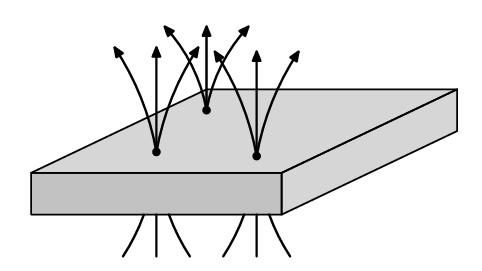
\includegraphics[width=0.8\linewidth]{Immagini/Superconductivity_images/Type_2_vortices.jpg}
	\caption{Vortices in a type II superconductor.}
	\label{vortici}
\end{figure}

\subsection{The London Equations}
The behaviour of the current density $\mathbf{J}$ in a superconducting material is described by the London equations:

\begin{align}
	\dfrac{\partial \mathbf{J}}{\partial t} &=  \dfrac{\mathbf{E}}{\mu_0 \lambda^2} \label{eq:London_1} \\
	\nabla \times \mathbf{J} &= - \dfrac{\mathbf{B}}{\mu_0 \lambda^2} \label{eq:London_2}
\end{align}
These equations characterize the electrodynamic response of superconductors. The parameter $\lambda$, known as the London penetration depth, measures how deeply a magnetic field can penetrate into the superconducting material. Using Maxwell’s equations, one can show that the London equations are equivalent to:
\begin{align}
	\mathbf{J} = - \dfrac{\mathbf{A}}{\mu_0 \lambda^2}
	\label{eq:London:gauge}
\end{align}
where the vector potential $\mathbf{A}$ plays the role of the electric field $\mathbf{E}$ in the constitutive relation \ref{eq:Ohm}. 

London equations can be used to explain the Meissner effect. By substituting Maxwell's \ref{eq:maxwell4} equation into equation \ref{eq:London:gauge}, the following equation is obtained
\begin{align*}
	\nabla \times ( \nabla \times \mathbf{B} ) = - \dfrac{\mathbf{B}}{\lambda^2}
\end{align*}
using the vector identity
\begin{align}
	\nabla \times (\nabla \times \mathbf{A}) = \nabla (\nabla \cdot \mathbf{A}) - \nabla^2 \mathbf{A}
\end{align}
and using Maxwell's equation \ref{eq:maxwell3}, the following equation is obtained
\begin{align}
	\nabla^2 \mathbf{B} = \dfrac{\mathbf{B}}{\lambda^2}
\end{align}
By solving this equation one can see that in the pure superconducting state the only field allowed is exponentially damped going in from an external surface. Consider for example a semi-infinite superconductor occupying the space on the positive side of the $x$ axis with a uniform filed as in figure \ref{Penetration_x}.
\begin{figure}[H]
	\centering
	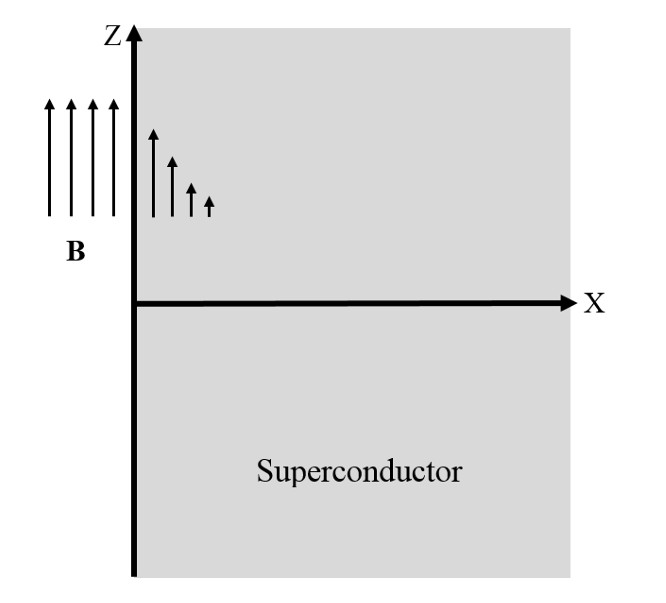
\includegraphics[width=0.5\linewidth]{Immagini/Superconductivity_images/Penetrazion_x.jpg}
	\caption{}
	\label{Penetration_x}
\end{figure}
With this geometry, the previous equation reduces to the form:
\begin{align*}
	\dfrac{\partial^2B_z}{\partial x^2} = \dfrac{B_z}{\lambda^2}
\end{align*}
The only solution to this ODE that is consistent with the boundary condition $B_z(x=0) = B_0$ and with finite energy (calculated from equation \ref{energia_EM}) is 
\begin{align}
	B_z(x) = B_0e^{-\frac{x}{\lambda}}
\end{align}
this exponential decay of the magnetic field near the surface of a superconductor in the Meissner stateis illustrated in figure \ref{London_penetration}.
\begin{figure}[H]
	\centering
	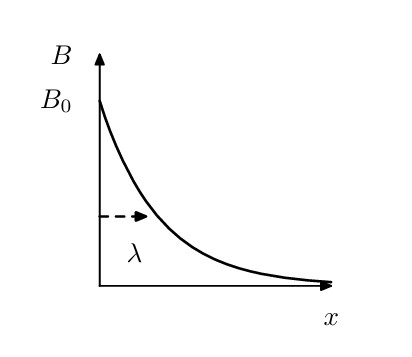
\includegraphics[width=0.55\linewidth]{Immagini/Superconductivity_images/London_depth.jpg}
	\caption{}
	\label{London_penetration}
\end{figure}

\subsection{The Ginzburg-Landau model}
The Ginzburg-Landau model is a fenomenological theory that describes the superconductive phase transition from a thermodinamical perspective and it can be shown that it follows from the BCS theory.
When describing a phase transition an order parameter, is a variable that is zero when the transition has not happened and is different from zero when the transition has happened, an example of this is the spontaneus magnetization of a ferromegnetic material below its Curie temperature. The assumpion of the Ginzburg-Landau theory is that a superconductive material is described by a complex order parameter $\psi$ such that  
\begin{align}
	\psi = \begin{cases}
		0 & T > T_c\\ 
		\psi (T) \neq 0 & T < T_C
	\end{cases}
\end{align}
Further more, it assumes that the Helmholtz free energy of the superconductor (defined as $F=U -TS$) depends smoothly on the parameter $\psi$. Since $\psi$ is complex and the free energy must be real, the energy can only depend on $|\psi|$. Since $\psi$ goes to zero at the critical temperature $T_c$, the free energy can be expanded in powers of $|\psi|$. For temperatures close to $T_c$ only the first two terms in the expansion should be necessary, and so the free energy density ($f = F/V$) must be of the form:
\begin{align}
	f_s(T) \approx f_n(T) + a(T) |\psi|^2 +\dfrac{1}{2}b(T) |\psi|^4 
	\label{eq:landau_free_energy_const}
\end{align}
Here $f_s(T)$ and $f_n(T)$ are the superconducting state and normal state free energy densities, respectively. Equation \ref{eq:landau_free_energy_const} is the only possible function which is real for any complex $\psi$ near $\psi=0$ and which is a differentiable function of $\psi$ and $\psi^*$ near to $\psi = 0$. The parameters $a(T)$ and $b(T)$ are, in general, temperature dependent pheonomenological parameters of the theory. However it is assumed that they must be smooth functions of temperature. The theory also assumes that $b(T)$ is positive, since otherwise the free energy density would have no minimum, which would be unphysical (or we would have to extend the expansion to include higher powers such as $|\psi|^6$). Plotting $f_s - f_n$ as a function of $|\psi|$ is easy to see that there are two possible curves, depending on the sign of the parameter $a(T)$, as shown in figure. In the case $a(T) < 0$, the curve has one minimum at $\psi = 0$. On the other hand, for $a(T) < 0$ there are minima wherever $|\psi|^2 = -\frac{a(T)}{b(T)}$. The model assumes that at high temperatures, above $T_c$, we have $a(T)$ positive, and hence the minimum free energy solution is one with $\psi = 0$, namely the normal state. But if $a(T)$ gradually decreases as the temperature $T$ is reduced, then the state of the system will change suddenly when we reach the point $a(T) = 0$. Below this temperature the minimum free energy solution changes to one with $\psi = 0$. Therefore the temperature where $a(T)$ becomes zero can be identified as the critical temperature $T_c$.
\begin{figure}[H]
	\centering
	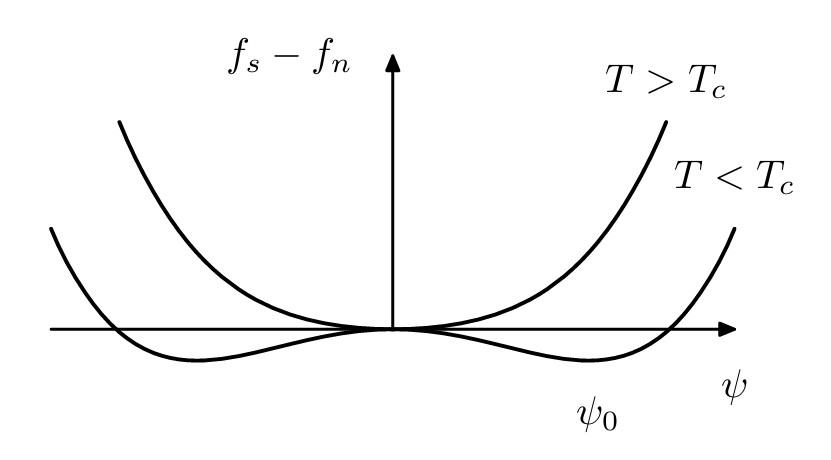
\includegraphics[width=0.7\linewidth]{Immagini/Superconductivity_images/Landau_gobba.jpg}
	\caption{Free energy difference between the normal and superconducting states (per unit volume) as a function of the order parameter $\psi$. For $T < T_c$ the free energy has a minimum at $\psi_0$, while for T > Tc the only minimum is at $\psi = 0$.}
	\label{Landau_free_energy}
\end{figure}

The complete Ginzburg-Landau theory of superconductivity also allows for the possibility that the order parameter depends on position $\psi(\mathbf{r})$. The theory postulates that the free energy is as given above, together with a new term depending on the gradient of $\psi(\mathbf{r})$. With this term free energy density becomes:
\begin{align}
	f_s(T) = f_n(T) + \dfrac{\hbar^2}{2m^*}|\nabla \psi (\mathbf{r})|^2 + a(T) |\psi (\mathbf{r})|^2 +\dfrac{b(T)}{2} |\psi (\mathbf{r})|^4
	\label{Eq:free_energy_noB}
\end{align}
The new parameter $m^*$ determines the energy cost associated with gradients in $\psi(\mathbf{r})$. It has dimensions of mass, and it plays the role of an effective mass for the quantum system with macroscopic wave function $\psi(\mathbf{r})$.

In order to find the order parameter at the equilibrium, one must minimize the total free energy of the system:
\begin{align}
	F_s(T) = F_n(T) + \int \bigg( \dfrac{\hbar^2}{2m^*}|\nabla \psi (\mathbf{r})|^2 + a(T) |\psi (\mathbf{r})|^2 +\dfrac{b(T)}{2} |\psi (\mathbf{r})|^4 \bigg) d^3 \mathbf{r}
\end{align}
To find the minimum, the infinitesimal change in the total free energy $\delta F$ must be equal to zero for any change in the order parameter $\delta \psi$. This leads to the following equation:
\begin{align}
	-\dfrac{\hbar^2}{2m^*} \nabla^2 \psi + a \psi + b \psi |\psi|^2 = 0
	\label{eq:schrod_eff}
\end{align}
This is a Schrödinger-like equation that allows us to find the order parameter $\psi(\mathbf{r})$ in equilibrium conditions.  However, unlike the usual Schrödinger equation, this is a non-linear equation because of the second term in the bracket and because of this non-linearity the principle of superposition does not apply. 

The effective non-linear Schrödinger equation \ref{eq:schrod_eff} can be used to study the response of the superconducting order parameter to external perturbations. Considering a simple model for the interface between a normal metal and a superconductor with the interface liyng in the $yz$ plane separating the normal metal in the $x < 0$ region from the superconductor in the $x > 0$ region. On the normal metal side of the interface the superconducting order parameter, $\psi (\mathbf{r})$, must be zero. Assuming that $\psi (\mathbf{r})$ must be continuous leads to the following non-linear Schrödinger equation
\begin{align}
	-\dfrac{\hbar^2}{2m^*} \dfrac{d^2\psi}{dx^2} + a \psi + b \psi |\psi|^2 = 0
	\label{eq:schrod_eff_1D}
\end{align}
in the region $x > 0$ with the boundary condition $\psi(0) = 0$. This equation can be solved directly and its solution is
\begin{align}
	\psi(x) = \psi_0 \tanh \bigg( \dfrac{x}{\sqrt{2} \xi(T)} \bigg)
\end{align}
as shown in figure \ref{Landau_Coerence_lenght}.

\begin{figure}[H]
	\centering
	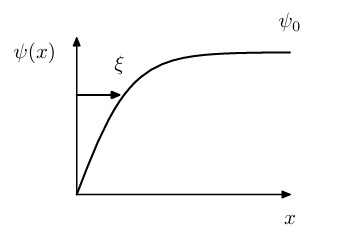
\includegraphics[width=0.6\linewidth]{Immagini/Superconductivity_images/Coerenza.jpg}
	\caption{Order parameter of a superconductor near a surface. It recovers to its bulk value $\psi_0$ over a length scale of the coherence length, $\xi$.}
	\label{Landau_Coerence_lenght}
\end{figure}
Here $\psi_0$ is the value of the order parameter in the bulk far from the surface and the parameter $\xi(T)$ id defined by
\begin{align}
	\xi(T) = \dfrac{\hbar}{\sqrt{2m^*|a(T)|}}
\end{align}
This quantity, which has dimensions of length, is called the Ginzburg-Landau coherence length. It is an important physical parameter characterizing the superconductor. In figure \ref{Landau_Coerence_lenght} one can see that $\xi(T)$ is a measure of the distance from the surface over which the order parameter has recovered back to nearly its bulk value.

In the presence of a magnetic field the expression \ref{Eq:free_energy_noB} ,ust be extended according to the minimal substitution:
\begin{align}
	-i \hbar \nabla \rightarrow  - i \hbar \nabla -q \mathbf{A}
\end{align}
For all known superconductors it turns out that the appropriate charge $q$ is $-2e$ and the reason for this becomes clear in the BCS theory. With this replacement the Ginzburg-Landau free energy density of the superconductor becomes
\begin{align}
	f_s(T) = f_n(T) + \dfrac{1}{2m^*}|(-i \hbar\nabla +2e \mathbf{A}) \psi |^2 + a |\psi|^2 +\dfrac{b}{2} |\psi (\mathbf{r})|^4
	\label{Eq:free_energy_B}
\end{align}
and the total free energy of the sistem becomes
\begin{align}
	F_s(T) = F_n(T) + \int \bigg( \dfrac{1}{2m*} |(-i\hbar \nabla +2e \mathbf{A}) \psi|^2 + a|\psi|^2 + \dfrac{b}{2} |\psi|^4 \bigg) d^3 \mathbf{r}
\end{align}
again, imposing $\delta F =0$ for any $\delta \psi$ leads to the effective Schrödinger equation:
\begin{align}
	\dfrac{1}{2m^*} (-i \hbar\nabla + 2e\mathbf{A})^2\psi + a \psi + b \psi |\psi|^2 = 0
	\label{eq:schrod_eff_B}
\end{align}

The London equation \ref{eq:London:gauge} can be shown to follow from the Ginzburg-Landau model. This can be done using the following expression for the current density:
\begin{align}
	\mathbf{J} = - \dfrac{\partial F}{\partial \mathbf{A}}
	\label{eq_landau_supercurrent}
\end{align}
where is the functional derivative, which is defined by the relation:
\begin{align}
	\delta F = \int \dfrac{\partial F}{\partial \mathbf{A}} \cdot \delta \mathbf{A} \, d^3 \mathbf{r}
	\label{eq:functional_derivative}
\end{align}
This equation gives:
\begin{align}
	\mathbf{J} = - \dfrac{\partial F}{\partial \mathbf{A}} = -\dfrac{e \hbar i}{m^*} (\psi^* \nabla \psi - \psi \nabla \psi^*) - \dfrac{4e^2}{m^*} |\psi|^2 \mathbf{A}
\end{align}
in the bulk of the material the order parameter can be considered uniform, therefore $\nabla \psi = \nabla \psi^* = \mathbf{0}$ and we can write
\begin{align}
	\mathbf{J} = - \dfrac{4e^2|\psi|^2}{m^*} \mathbf{A}
\end{align}
which is the London equation \ref{eq:London:gauge}. Comparing this with the known form, it follows that:
\begin{align}
	m^* = 2m_e
\end{align}
and
\begin{align}
	|\psi|^2 = \dfrac{n_s}{2}
\end{align}
where $n_s$ is the electron density. This gives a hint for the physical meaning of the order parameter $\psi$ and the effective mass $m^*$: $\psi$ is the coherent wave function of the Cooper pairs and $m^*$ is the mass of a single Cooper pair.

\subsection{The BCS theory}
The Ginzburg–Landau model makes it clear that the superconducting phase must originate from a coupling mechanism between electrons, as the phenomenological parameters take the values $q = -2e$ and $m^* = 2m_e$. However, the model itself does not explain the nature of this coupling. The BCS theory accounts for superconductivity by introducing an attractive interaction between electrons mediated by the exchange of lattice phonons. As an electron moves through the crystal, it distorts the lattice by attracting nearby ions, creating a region of increased positive charge density. This region, in turn, attracts another electron, forming a bound state known as a Cooper pair. Figure \ref{fig:Feynmann_Phonon} shows the Feynman diagram corresponding to this interaction.
\begin{figure}[H]
	\centering
	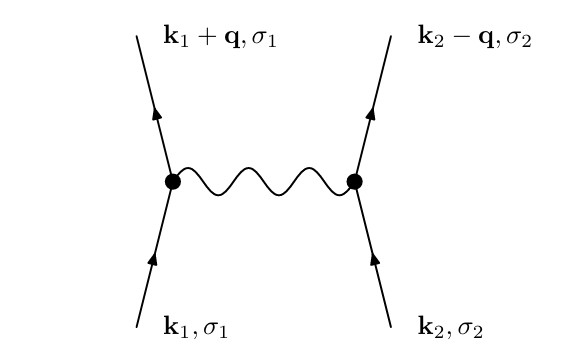
\includegraphics[width=0.6\linewidth]{Immagini/Superconductivity_images/Feynmann_phonon.jpg}
	\caption{Feynmann diagram representing the interaction between electrons at the Fermi surface due to exchange of crystal lattice phonons.}
	\label{fig:Feynmann_Phonon}
\end{figure}
The time is represented in the vertical axis, while the space is represented in the horizontal axes.

This effective interaction between the electrons due to exchange of phonons is of the form:
\begin{align*}
	V_{eff}(\mathbf{q},\omega) = \dfrac{|g_{\mathbf{q}}|^2}{\omega^2-\omega_{\mathbf{q}}^2}
\end{align*}
Where the phonon has wave vector $\mathbf{q}$ and frequency $\omega$. The parameter $g_{\mathbf{q}}$ is related to the matrix element for scattering an electron from state $\mathbf{k}$ to $\mathbf{k}+\mathbf{q}$ as shown in figure \ref{fig:Feynmann_Phonon} and is of the order
\begin{align*}
		g_{\mathbf{q}} \sim \sqrt{\dfrac{m}{M}}
\end{align*}
where $m$ is the effective mass of the electrons at he Fermi surface and $M$ is the mass of the lattice ions. Since $\frac{m}{M}$ is of order $10^{-4}$, typically, the electrons and phonons are only weakly coupled, this entails that all the diagrams of higher order than the one in figure \ref{fig:Feynmann_Phonon} (that involve more vertices) can be neglected. By neglecting the dependence of the interaction the wave vector and replacing the interaction with an approximate one that effectively averages over all values of $\mathbf{q}$, it takes the form:
\begin{align*}
		V_{eff}(\mathbf{q},\omega) = \dfrac{|g_{eff}|^2}{\omega^2-\omega_D^2}
\end{align*}
where $\omega_D$ is the Debye frequency of phonons. This interaction only involves electrons in a thin shell of thickness $2 \hbar \omega_D$ around the Fermy surface (shown in figure \ref{fig:Fermi_surface_1}), since only these states can change energy without violating the Pauli exclusion principle.
\begin{figure}[H]
	\centering
	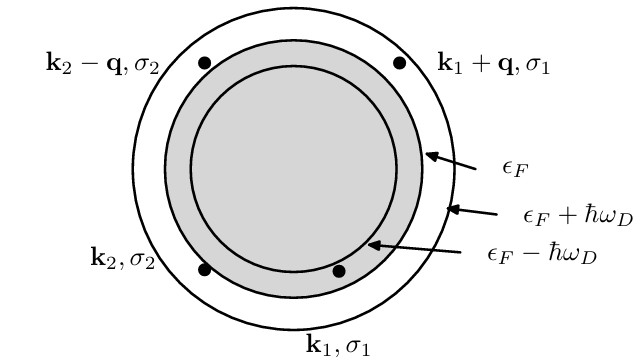
\includegraphics[width=0.7\linewidth]{Immagini/Superconductivity_images/Fermi_surface_1.jpg}
	\caption{The effective electron-electron interaction near the Fermi surface.}
	\label{fig:Fermi_surface_1}
\end{figure}
Since $\hbar \omega_D << K_B T$ the interaction is always attractive and it can be approximated as: 
\begin{align}
	V_{eff} = -|g_{eff}|^2
\end{align} 
The corresponding effective Hamiltonian for the effective electron-electron interaction is therefore:
\begin{align}
	H = -|g_{eff}|^2 \sum c_{\mathbf{k_1} + \mathbf{q}, \sigma_1}^{\dagger} c_{\mathbf{k_2} - \mathbf{q}, \sigma_1}^{\dagger} c_{\mathbf{k_1}, \sigma_1} c_{\mathbf{k_2}, \sigma_2}^{\dagger}
\end{align}
where $c_{\mathbf{k}, \sigma}^{\dagger}$ and $c_{\mathbf{k}, \sigma}$ respectively denote the creation and distruction operator of an electron with momentum $\mathbf{k}$ and spin $\sigma$ respectively. The sum is over all values of $\mathbf{k_1}$, $\sigma_1$, $\mathbf{k_2}$, $\sigma_2$ and $\mathbf{q}$ with the restriction that the electron energies involved are all within the range $\pm \hbar \omega_D$ of the Fermi surface as in figure \ref{fig:Fermi_surface_1}.

The wave function for a pair of electrons near the Fermi surface can be written as:
\begin{align*}
	\Psi (\mathbf{r}_1, \sigma_1, \mathbf{r}_2, \sigma_2) = e^{\mathbf{k}_c \cdot \mathbf{R}} \varphi (\mathbf{r}_1 - \mathbf{r}_2) \phi^{spin}_{\sigma_1, \sigma_2}
	\label{eq:Cooper_pair_wave_function}
\end{align*} 
where $\mathbf{R}$ and $\mathbf{k}_c$ are the position and momentum of the center of mass respectively. In the ground state $\mathbf{k}_c = 0$ and in most superconductors, the pair is in a singlet state: 
\begin{align*}
	\phi^{spin}_{\sigma_1, \sigma_2} = \dfrac{1}{\sqrt{2}} (\ket{\uparrow \downarrow} - \ket{\downarrow \uparrow})
\end{align*}
therefore, since electrons are fermions and their wave functions must be antisimmetrical, $ \varphi (\mathbf{r}_1 - \mathbf{r}_2)$ must be an even function. Substituting the wave function \ref{eq:Cooper_pair_wave_function} into the Schrödinger's equation gives the following expression for the energy of a Cooper pair:
\begin{align}
	E = - 2 \hbar \omega_D e^{-\frac{1}{\lambda}}
\end{align}
with:
\begin{align*}
	\lambda = |g_{eff}|^2 g(\varepsilon_F)
\end{align*}
where $g(\varepsilon_F)$ is the density of state evaluated at the Fermi level. This confirms the existence of a bound state between two electrons at the fermi surface. This entails that the entire Fermi surface is unstable to the creation of Cooper pairs. The wave function on the entire system is given by the coherent wave function:
\begin{align*}
	\ket{\Psi_{\text{BCS}}} = C \, \text{exp} \left( \sum_{\mathbf{k}} \alpha_{\mathbf{k}} P_{\mathbf{k}^{\dagger}} \right) \ket{0}
\end{align*} 
where
\begin{align}
	P_{\mathbf{k}}^{\dagger} = c_{\mathbf{k} \uparrow}^{\dagger} \, c_{\mathbf{-k} \downarrow}^{\dagger}
\end{align}
is the operator that creates a Cooper pair and $\ket{0}$ is the vacuum state where no Cooper pair is present. Using the properties of the creation and destruction operators (the calculations are shown in \cite{Annet}) the wave function can be rewritten as:
\begin{align}
	\ket{\Psi_{\text{BCS}}} = \prod_{\mathbf{k}} \left( u_{\mathbf{k}}^* + v_{\mathbf{k}}^* P_{\mathbf{k}}^{\dagger}\right) \ket{0}
\end{align}
where
\begin{align*}
	u_{\mathbf{k}}^* = \dfrac{1}{1+|\alpha_{\mathbf{k}|^2}}
\end{align*}
\begin{align*}
	v_{\mathbf{k}}^* = \dfrac{\alpha_{\mathbf{k}}}{1+|\alpha_{\mathbf{k}|^2}}
\end{align*}
The values of $u_{\mathbf{k}}^*$ and $v_{\mathbf{k}}^*$	can be found using the variational method and minimizing the energy functional
\begin{align*}
	E = \bra{\Psi_{\text{BCS}}} H \ket{\Psi_{\text{BCS}}}
\end{align*} 
This procedure gives the following system of equations:
\begin{empheq}[left=\empheqlbrace]{align*}
	& |u_{\mathbf{k}}|^2 = \dfrac{1}{2} \left( 1 + \dfrac{\varepsilon_{\mathbf{k}} - \mu}{E_{\mathbf{k}}} \right) \\
	& |v_{\mathbf{k}}|^2 = \dfrac{1}{2} \left( 1 - \dfrac{\varepsilon_{\mathbf{k}} - \mu}{E_{\mathbf{k}}} \right) \\
	&  E_{\mathbf{k}} = \sqrt{(\varepsilon_{\mathbf{k}} - \mu)^2 + |\Delta|^2} \\
	& \Delta = |g_{eff}|^2 = \sum_{\mathbf{k}} u_{\mathbf{k}} v_{\mathbf{k}}^*
\end{empheq}
where $\Delta$ is called the BCS gap parameter. The system leads to the following expression for the gap parameter at $T=0$:
\begin{align}
	|\Delta| = 2 \hbar \omega_D e^{-\frac{1}{\lambda}}
\end{align}
From this, the expression for the gap parameter at finite temperature can be obtained by taking $\ket{\Psi_{\text{BCS}}}$ as the reference state and considering small excitations relative to it. The resulting formula follows from expressing the creation and distruction operators in terms of the quasiparticle creation and distruction operators and using their Fermi–Dirac occupation statistics.

\newpage

\section{Proximity Effects}

\subsection{Superconductor-Ferromagnet Interfaces}
Due to their opposite ordering, ferromagnetism and superconductivity are highly incompatible: the exchange field, in a magnetically ordered state, tends to align the spins of the Cooper pairs in the same direction, thus preventing a pairing effect, this is called paramagnetic effect. Because of this effect,  the coexistence of singlet superconductivity with ferromagnetism is very unlikely in bulk materials.

However, at the interface between a ferromagnetic and a superconducting material, the Cooper pairs can penetrate the ferromagnet at some distance and induce superconducting-like properties (this phenomenon is called proximity effect), at the same time the leakage of the Cooper pairs weakens the superconductivity near the interface (this effect is called the inverse proximity effect). These effects result in a decrease of the superconducting transition temperature in a thin superconducting layer. If the thickness of a superconducting layer is smaller than a critical one, the proximity effect totally suppresses the superconducting transition. This effect causes the coherent wave function $\psi$ in the ferromagnet (that is associated to the cooper pairs that crossed the interface) to decay exponantially, as in a superconductor-metal interface, but modulated by an additional oscillating factor due to the exchange field.

The oscillatory behavior of the order parameter can be understood qualitatively using the generalized Ginzburg–Landau theory, in analogy with the treatment of the FFLO state in \cite{Proximity}. The free-energy density in the ferromagnet may be written as: 
\begin{align}
	f_s = f_n + a(H,T) |\psi|^2 + \gamma (H,T) |\nabla \psi|^2 + \dfrac{\eta (H,T)}{2} |\nabla ^2 \psi|^2 + \dfrac{b (H,T)}{2} |\psi|^4
\end{align}
By minimizing $f_s$ and chosing the $x$ axis perpendicular to the interface (so that $\psi$ depends only on $x$), the following equation for the order parameter $\psi$ is obtained:
\begin{align*}
	a \psi - \gamma \dfrac{\partial^2 \psi}{\partial x^2} + \dfrac{\eta}{2} \dfrac{\partial^4 \psi}{\partial x^4} = 0  
\end{align*}
the solutions to this equation are of the form:
\begin{align*}
	\psi = \psi_0 e^{kx}
	\label{eq:proximity_wave_function}
\end{align*}
with a complex wave vector $k$ given by:
\begin{align*}
	k = k_1 + i k_2
\end{align*}
and 
\begin{align*}
	k_1^2 = \dfrac{|\gamma|}{2 \eta} \left( \sqrt{1+ \dfrac{T-T_{ci}}{T_{ci}-T_{cu}}} -1 \right)
\end{align*}
\begin{align*}
	k_1^2 = \dfrac{|\gamma|}{2 \eta} \left( \sqrt{1+ \dfrac{T-T_{ci}}{T_{ci}-T_{cu}}} +1 \right)
\end{align*}
where $T_{cu}(H)$ is the critical temperature of the transition into the uniform superconducting state and $T_{ci}(H) > T_{cu}(H)$ is critical temperature of the non-uniform (FFLO-type) superconducting state. These temperatures are effective parameters describing the hypothetical superconducting state associated with the wave function $\psi$ in the ferromagnetic region. Chosing $\psi$ to be real leads the following expression:
\begin{align}
	\psi (x) = \psi_i e^{-k_1 x} \text{cos} (k_2 x)
\end{align}
The behaviour of the order parameter $\psi$ in the ferromagnet is sketched in figure \ref{S_F_Landau}.
\begin{figure}[H]
	\centering
	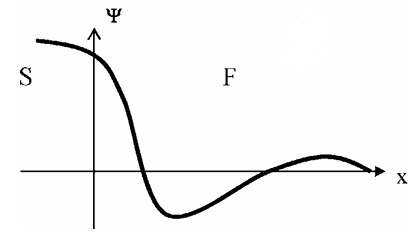
\includegraphics[width=0.6\linewidth]{Immagini/Proximity_images/S_F_Landau.jpg}
	\caption{Schematic behavior of the superconducting order parameter near the  superconductor-ferromagnet interface.}
	\label{S_F_Landau}
\end{figure}
This oscillating behaviour is a fundamental difference between the proximity effect in superconductor-ferromagnet and superconductor-metal systems, and it is at the origin of many peculiar characteristics of superconductor-ferromagnet heterostructures.
\newpage

\subsection{Shift in the resonant field}
The first evidence for a shift in the FMR resonant frequency (and field) in superconductor–ferromagnet–superconductor trilayers is presented in \cite{First_Evidence_1}, \cite{First_Evidence_2}, and \cite{Magnetization}. Figure \ref{Sample_Geometry} shows a schematic representation of the trilayers used in these works, together with the static (DC) and oscillating (mw) magnetic fields employed in the FMR measurements.
\begin{figure}[H]
	\centering
	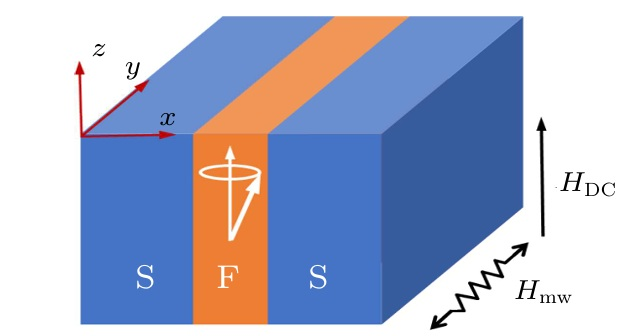
\includegraphics[width=0.8\linewidth]{Immagini/Proximity_images/Sample_Geometry.jpg}
	\caption{Geometry of the ferromagnetic Josephson junctions and configuration of FMR measurements.}
	\label{Sample_Geometry}
\end{figure}
These studies show that when FMR measurements are conducted on an S/F/S thin-film trilayer, the resonant frequency and field no longer obey the standard Kittel equation \ref{eq:Kittel}. Instead, they follow the modified Kittel equation:
\begin{align}
	\omega_{res} = \gamma \sqrt{(H_{res}+H_a)(H_{res}+H_a+M_{eff})}
	\label{eq:Kittel_modified}
\end{align}
where $H_a$ is an additional anisotropy field. This equation indicates that the superconducting layers generate an effective magnetic field in the same direction as the external DC field, implying that a lower external field is required to reach ferromagnetic resonance. Figure \ref{Absorption_SFS} shows the FMR absorption spectra measured in \cite{Magnetization} for a trilayer sample above and below the critical temperature.

\begin{figure}[h]
	\centering
	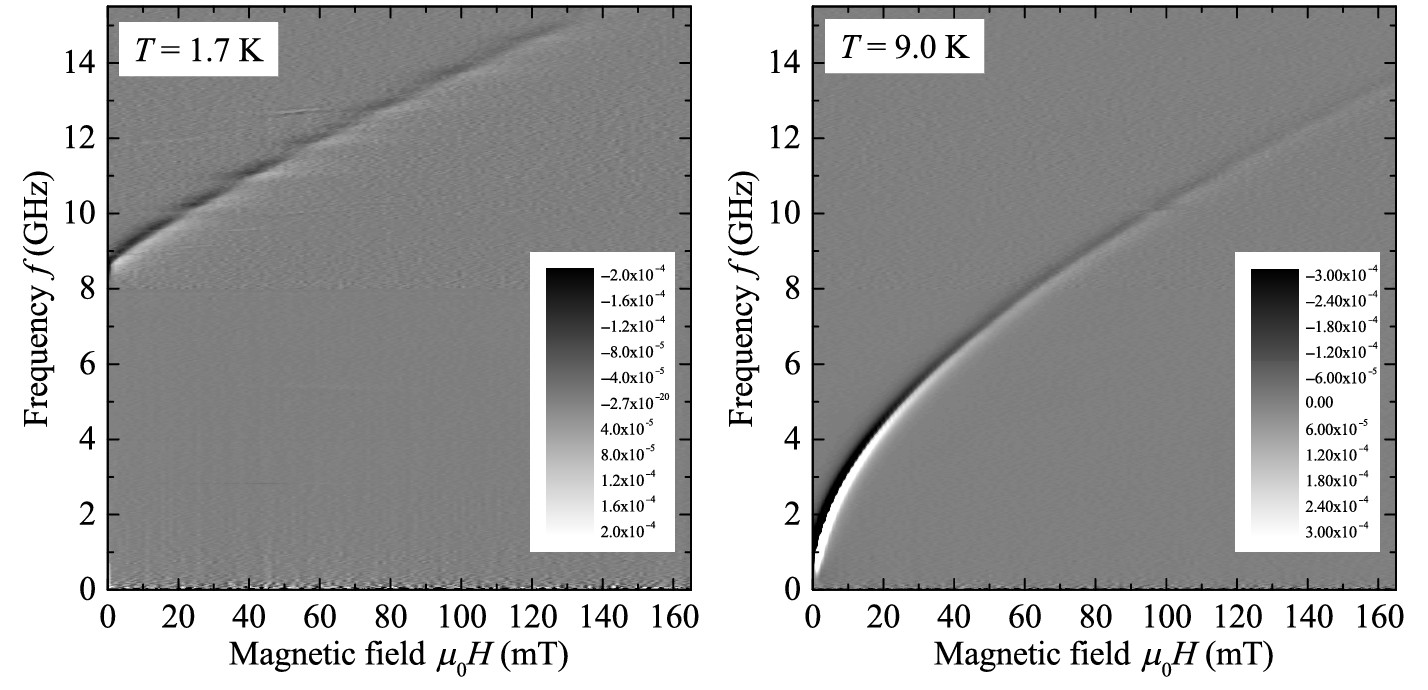
\includegraphics[width=\linewidth]{Immagini/Proximity_images/Assorbimento_SFS.jpg}
	\caption{FMR absorption spectra for a sample above and below the critical temperature for a S(Nb$=110$ nm)F(Py$=19$ nm)S(Nb$=110$ nm) trilayer sample. The grayscale is coded in absolute units.}
	\label{Absorption_SFS}
\end{figure}

In both graphs, the line corresponding to the maximum absorption (resonance) is clearly visible, and for the same frequency the corresponding resonant field is lower at $T = 1.7$ K than at $T = 9.0$ K. Figure \ref{First_Shift} shows the results of a similar experiment performed in \cite{First_Evidence_1} on another trilayer sample made of the same materials and grown on a SiO$_2$ substrate. The upper panel shows the absorption spectra at different temperatures above and below the critical temperature of the superconducting layers. As explained in the next chapter, the experimental setup measures a voltage proportional to the derivative of the absorbed power with respect to the DC external magnetic field; therefore, the plotted data correspond to the derivative of a Lorentzian. The lower panel shows the resonant fields extracted from these data as a function of temperature, along with a schematic representation of the sample.

\begin{figure}[h]
	\centering
	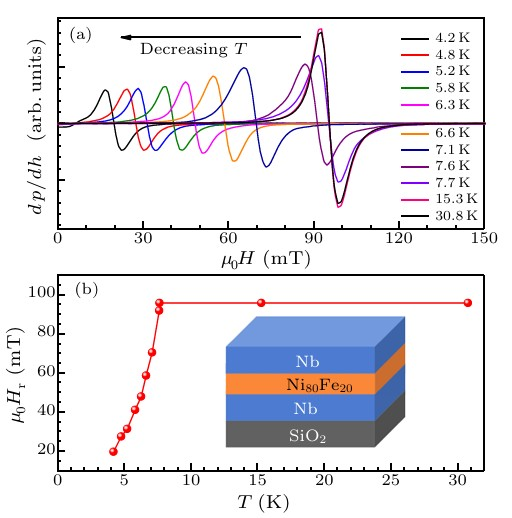
\includegraphics[width=0.7\linewidth]{Immagini/Proximity_images/First_Shift_Hres.jpg}
	\caption{FMR spectra of a Nb(100 nm)/Ni${80}$Fe${20}$(20 nm)/Nb(100 nm) Josephson junction. (a) FMR spectra at various temperatures. Below the superconducting transition temperature $T_c$, the resonance field $H_r$ shifts to lower values with decreasing temperature. (b) Resonance field $H_r$ as a function of temperature. The inset shows the sample structure.}
	\label{First_Shift}
\end{figure}

All the resonance lines exhibit a single Lorenz lineshape. The resonant field changes little with temperature above $T_c$. However, it shifts rapidly to a lower field with decreasing temperature below $T_c$. and the significant shift of $H_r$ below the critical temperature demonstrates a strong proximity-induced modification of the magnetization dynamics caused by superconductivity.

Furthermore, these studies attempt to identify the mechanism responsible for this effect. More specifically, they investigate whether the additional anisotropy field is generated by supercurrents flowing through the entire Josephson junction rather than by a local proximity effect at a single S/F interface. If this hypothesis is correct, no shift should be observed in an S/F bilayer, nor in an S/I/F/S multilayer (where an insulating layer prevents Josephson coupling). Finally, an S/F/S/F multilayer should behave as a combination of an S/F/S trilayer and an S/F bilayer: above $T_c$ the system should exhibit a single resonance line (because the two structures share the same resonant field and frequency), whereas below $T_c$ two distinct lines should appear (since the resonant field shifts only in the trilayer). These experiments were performed in \cite{First_Evidence_1}, and the results are shown in Fig. \ref{Control}.

\begin{figure}[h]
	\centering
	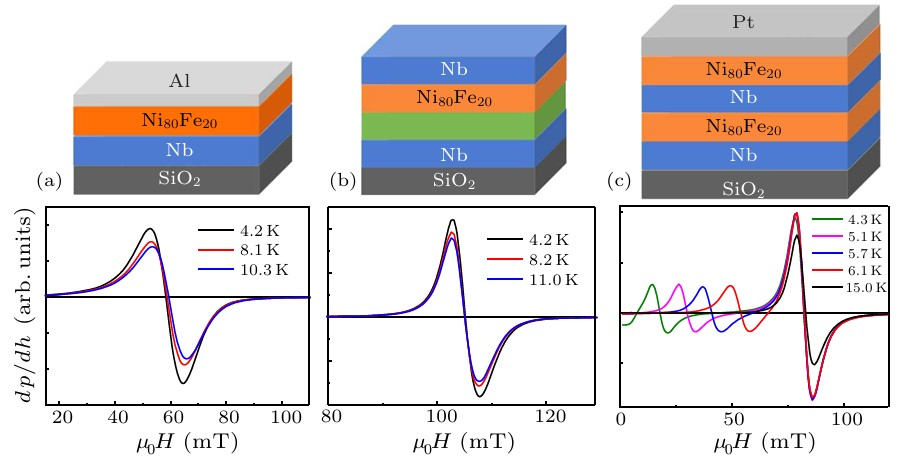
\includegraphics[width=0.9\linewidth]{Immagini/Proximity_images/Control.jpg}
	\caption{Control experiments on S/F bilayer, S/I/F/S, and S/F/S/F multilayers. (a) FMR spectra of a Nb(100 nm)/Ni${80}$Fe${20}$(20 nm) bilayer, showing no shift below $T_c$. (b) FMR spectra of a Nb(100 nm)/MgO(10 nm)/Ni${80}$Fe${20}$(20 nm)/Nb(100 nm) multilayer, again without a shift below $T_c$. (c) FMR spectra of a Nb(100 nm)/Ni${80}$Fe${20}$(20 nm)/Nb(100 nm)/Ni${80}$Fe${20}$(20 nm) multilayer. Above $T_c$ there is a single resonance line, whereas below $T_c$ two distinct lines appear: the upper NiFe layer shows no shift, while the lower NiFe layer in the S/F/S junction shifts to lower fields.}
	\label{Control}
\end{figure}

These experiments confirmed the hypothesis: no resonant-field shift was detected in the S/F bilayer nor in the S/I/F/S multilayer, while the S/F/S/F multilayer exhibited one resonance line above $T_c$ and two below $T_c$. Overall, these results demonstrate that the shift of the resonant field below the critical temperature occurs only in conducting ferromagnetic Josephson junctions.

In \cite{Magnetization} it is shown that the dependence of the anisotropy field $H_a$ on the temperature can be characterized by fitting it with the following power law expression:
\begin{align}
	H_a(T) = H_0 \left( 1- \left( \dfrac{T}{T_c} \right)^p \,\right)
	\label{eq:power_law}
\end{align}
where $H_0$ is the effective anisotropy field at zero temperature, $T_c$ is the critical temperature, and $p$ is a free exponent parameter. The fit of $H_a(T)$ with equation \ref{eq:power_law} is shown in figure \ref{Anisotropy_fit}.

\begin{figure}[h]
	\centering
	    \begin{minipage}{0.45\textwidth}
		\centering
		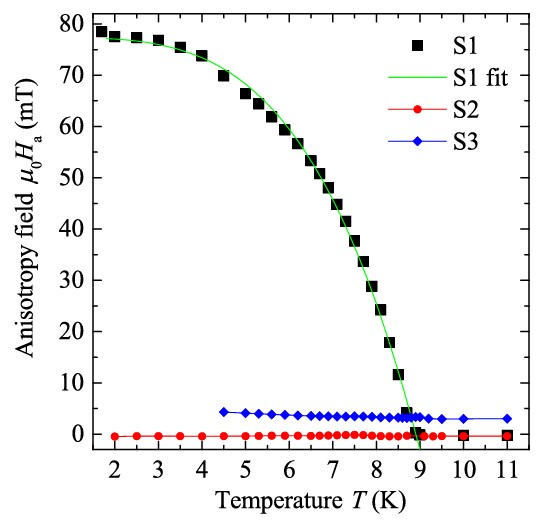
\includegraphics[width=\linewidth]{Immagini/Proximity_images/Anisotropy_fit.jpg}
		\label{fig:img1}
	\end{minipage}
	\hfill
	\begin{minipage}{0.45\textwidth}
		\centering
		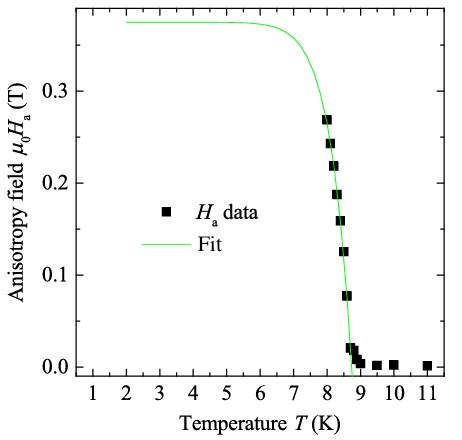
\includegraphics[width=\linewidth]{Immagini/Proximity_images/Anisotropy_fit_2.jpg}
		\label{fig:img2}
	\end{minipage}
	\caption{Temperature dependence of the anisotropy field. In the left image, black squares correspond to a symmetric S/F/S sample, red circles to an S/F/S sample with one significantly thinner superconducting layer, and blue diamonds to an S/F/I/S sample. The green curve shows the fit using equation \ref{eq:power_law}. In the right image, black squares correspond to another symmetric S/F/S sample, and the green curve represents the corresponding fit.}
	\label{Anisotropy_fit}
\end{figure}

However, the exact physical mechanism responsible for this shift remained unclear. According to \cite{First_Evidence_1}, the Meissner effect should be excluded because similar behavior would be expected in the S/I/F/S multilayer if flux focusing were the cause, as the thin MgO layer does not block magnetic flux. Since no shift is observed in such samples, the expulsion of external magnetic flux cannot explain the change in the ferromagnetic anisotropy. 

A possible explanation is presented in \cite{Russian}. According to this paper, the shift in the FMR resonant field is caused by the The Anderson-Higgs mechanism, which is a well known mechanism in high-energy and condensed matter physics in which particles acquire mass because of the spontaneus breking of gauge simmetry. In proximity coupled S/F/S trilayers, the spontaneous shift of the FMR frequency originates from an Anderson–Higgs–type mechanism that gives magnons a finite spectral gap and a mass. When the magnetization in the ferromagnetic layer precesses, its time-dependent magnetic flux induces curling electric fields in the adjacent superconductors, which in turn generate eddy supercurrents. As a result, magnons become massive, leading to a finite FMR frequency even at zero external magnetic field. This theory succesfully predicts some features of this phenomenon such as the occurence of the shift only in the presence of both the superconducting layers. 

The aim of this investigation is to reproduce the results obtained in \cite{First_Evidence_1}, \cite{First_Evidence_2}, and \cite{Magnetization}, and to verify whether this theoretical interpretation holds by conducting FMR measurements on S/F/S trilayers in different conditions.


\chapter{Experimental Methods and Setup}
In this investigation, a total of four experiments were conducted. The first two experiments aimed to reproduce the results reported in \cite{Magnetization} by demonstrating that the shift in the resonant field follows the behavior described in the paper: it appears only below a certain critical temperature (indicating its connection to superconductivity) and increases as the temperature decreases. These experiments also aimed to show that both superconducting layers are required for this effect to occur. This was verified by performing measurements on a sample containing only one superconducting layer. The remaining two experiments were designed to test the dynamic effect theory presented in \cite{Russian} by examining how the anisotropy field $H_a$ changes under different conditions: introducing an additional metallic layer between the ferromagnetic and superconducting layers and varying the microwave power.

\section{Sample fabrication}
The samples used in this study consisted of multilayer thin films with a layer of niobium (Nb), which is a type \RomanNumeralCaps{2} superconductor with a critical temperature of 9 K, a ferromagnetic layer of permalloy Ni$_{80}$Fe$_{20}$ (Py), followed by another niobium layer. The films were deposited on silicon (Si) substrates, which were cut into 5 mm $\times$ 5 mm squares and cleaned by sonication in acetone for 2 minutes, followed by sonication in isopropanol (IPA) for 2 minutes. This cleaning process is necessary to ensure a good adesion of the samples to the substrate and a uniform thickness of the samples and to make the experiment reproducible. In one of the experiment two copper (Cu) layers with variable thickness were introduced between both the superconducting and the ferromagnetic layers, figure \ref{Samples} shows the structure of the samples used in this experiment.
\begin{figure}[ht]
	\centering
	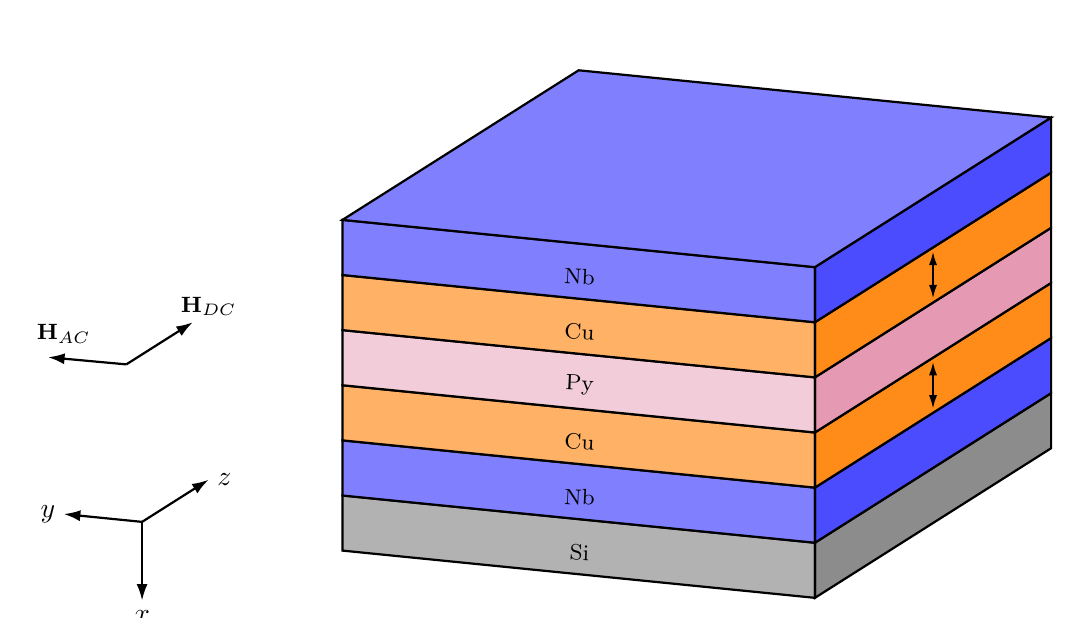
\begin{tikzpicture}[scale=1, thick]
		
		\fill[white] (-3,5) rectangle (3,5.25);
		
		% --- Si layer ---
		\fill[gray!60] (-3,0.6) -- (3,0) -- (3,0.7) -- (-3,1.3) -- cycle;
		\node[rotate=-atan(0.3/6), font=\footnotesize] at (0,0.35) [above] {Si};
		\fill[gray!90] (3,0) -- (6,1.9) -- (6,2.6) -- (3,0.7) -- cycle;
		\draw (3,0) -- (6,1.9) -- (6,2.6) -- (3,0.7) -- cycle; 
		\draw (-3,0.6) -- (3,0) -- (3,0.7) -- (-3,1.3) -- cycle;
		
		% --- Nb layer ---
		\fill[blue!50] (-3,1.3) -- (3,0.7) -- (3,1.4) -- (-3,2) -- cycle;
		\node at (0,1.05)[rotate=-atan(0.3/6), font=\footnotesize] [above] {Nb};
		\fill[blue!70] (3,0.7) -- (6,2.6) -- (6,3.3) -- (3,1.4) -- cycle;
		\draw (3,0.7) -- (6,2.6) -- (6,3.3) -- (3,1.4) -- cycle; 
		\draw (-3,1.3) -- (3,0.7) -- (3,1.4) -- (-3,2) -- cycle;
		
		% --- Cu layer ---
		\fill[orange!60] (-3,2) -- (3,1.4) -- (3,2.1) -- (-3,2.7) -- cycle;
		\node at (0,1.75)[rotate=-atan(0.3/6), font=\footnotesize] [above] {Cu};
		\fill[orange!90] (3,1.4) -- (6,3.3) -- (6,4) -- (3,2.1) -- cycle;
		\draw (3,1.4) -- (6,3.3) -- (6,4) -- (3,2.1) -- cycle; 
		\draw (-3,2) -- (3,1.4) -- (3,2.1) -- (-3,2.7) -- cycle;
		\draw[-{Latex[length=5pt,width=3pt]}] (4.5,2.7) -- (4.5,3);
		\draw[-{Latex[length=5pt,width=3pt]}] (4.5,2.7) -- (4.5,2.4);
		
		% --- Py layer ---
		\fill[purple!20] (-3,2.7) -- (3,2.1) -- (3,2.8) -- (-3,3.4) -- cycle;
		\node at (0,2.45)[rotate=-atan(0.3/6), font=\footnotesize] [above] {Py};
		\fill[purple!40] (3,2.1) -- (6,4) -- (6,4.7) -- (3,2.8) -- cycle;
		\draw (3,2.1) -- (6,4) -- (6,4.7) -- (3,2.8) -- cycle; 
		\draw (-3,2.7) -- (3,2.1) -- (3,2.8) -- (-3,3.4) -- cycle;
		
		% --- Cu layer ---
		\fill[orange!60] (-3,3.4) -- (3,2.8) -- (3,3.5) -- (-3,4.1) -- cycle;
		\node at (0,3.15)[rotate=-atan(0.3/6), font=\footnotesize] [above] {Cu};
		\fill[orange!90] (3,2.8) -- (6,4.7) -- (6,5.4) -- (3,3.5) -- cycle;
		\draw (3,2.8) -- (6,4.7) -- (6,5.4) -- (3,3.5) -- cycle; 
		\draw (-3,3.4) -- (3,2.8) -- (3,3.5) -- (-3,4.1) -- cycle;
		\draw[-{Latex[length=5pt,width=3pt]}] (4.5,4.1) -- (4.5,4.4);
		\draw[-{Latex[length=5pt,width=3pt]}] (4.5,4.1) -- (4.5,3.8);
		
		% --- Nb layer (top) ---
		\fill[blue!50] (-3,4.1) -- (3,3.5) -- (3,4.2) -- (-3,4.8) -- cycle;
		\node at (0,3.85)[rotate=-atan(0.3/6), font=\footnotesize] [above] {Nb};
		\fill[blue!70] (3,3.5) -- (6,5.4) -- (6,6.1) -- (3,4.2) -- cycle;
		\draw (3,3.5) -- (6,5.4) -- (6,6.1) -- (3,4.2) -- cycle; 
		\draw (-3,4.1) -- (3,3.5) -- (3,4.2) -- (-3,4.8) -- cycle;
		% --- Top parallelogram (closing face) ---
		\fill[blue!50] (-3,4.8) -- (3,4.2) -- (6,6.1) -- (0,6.7) -- cycle;
		\draw (-3,4.8) -- (3,4.2) -- (6,6.1) -- (0,6.7) -- cycle;
		
		% Magnetic fields
		\draw[-{Latex[length=6pt,width=4pt]}] (-4.9-0.8448, 3.5-0.5351) -- (-4.9-0.9950-0.8448, 3.5+0.090965-0.5351); % DC magnetic field
		\draw[-{Latex[length=6pt,width=4pt]}] (-4.9-0.8448, 3.5-0.5351) -- (-4.9, 3.5); % AC magnetic field
		\node at (-4.7, 3.7) {\footnotesize{$\mathbf{H}_{DC}$}};
		\node at (-4.7-0.9950-0.8448, 3.8+0.090965-0.5351) {\footnotesize{$\mathbf{H}_{AC}$}};
		
		% Cartesian coordinates
		\draw[-{Latex[length=6pt,width=4pt]}] (-4.7-0.8448, 1.5-0.5351) -- (-4.7-0.8448, 0.5-0.5351);
		\node at (-4.7-0.8448, 1.3-1.5351) {$x$};
		\draw[-{Latex[length=6pt,width=4pt]}] (-4.7-0.8448, 1.5-0.5351) -- (-4.7-0.8448-0.9950, 1.5-0.5351+0.0995); 
		\node at (-4.9-0.8448-0.9950, 1.5-0.5351+0.0995) {$y$};
		\draw[-{Latex[length=6pt,width=4pt]}] (-4.7-0.8448, 1.5-0.5351) -- (-4.7,1.5);
		\node at (-4.5,1.5) {$z$};
		
		\fill[white] (-3,-0.1) rectangle (3,-0.35);
		
	\end{tikzpicture}
	\caption{Scheme of the samples used in this study. The double arrows indicate the variable thickness of the copper layers. The figure also shows the orientation of the AC and DC magnetic fields used in the FMR measurements.}
	\label{Samples}
\end{figure}

These samples were grown by DC magnetron sputtering, a physical vapour deposition (PVD) technique widely employed for the fabrication of metallic and multilayer thin films because it ensures high deposition rates and uniform coatings. Furthermore it allowed to grow the different layers in the same process, thus avoiding the exposure of intermediate layers and ensuring a good interface quality. In this method described in detail in \cite{Sputtering}), an inert gas (argon in this case) is introduced into an ultra-high-vacuum chamber, and a high voltage is applied between the negatively charged target and the positively charged substrate. If the target material is conductive, then it is connected to direct current (DC) power supply and if the target material is insulator then it is connected to radio frequency (RF) power supply. Under the applied voltage, the gas is ionised, forming a plasma composed of positively charged ions and free electrons. The ions are accelerated by the electric field and strike the target with sufficient energy to eject atoms from it. These atoms then travel through the chamber and deposit as thin films on the substrate positioned in their path which is kept rotating to guarantee uniform sample thickness. In magnetron sputtering the plasma is confined near the target by a magnetic field that forces electrons to follow a helical trajectory around the magnetic field lines. This increases both the sputtering yield and the overall deposition efficiency. The properties of the deposited films can be ajusted by changing sputtering parameters such as gas pressure, target–substrate distance and system temperature. Figure \ref{Sputtering} illustrates the general scheme of a sputtering device. \\
\begin{figure}[ht]
	\centering
	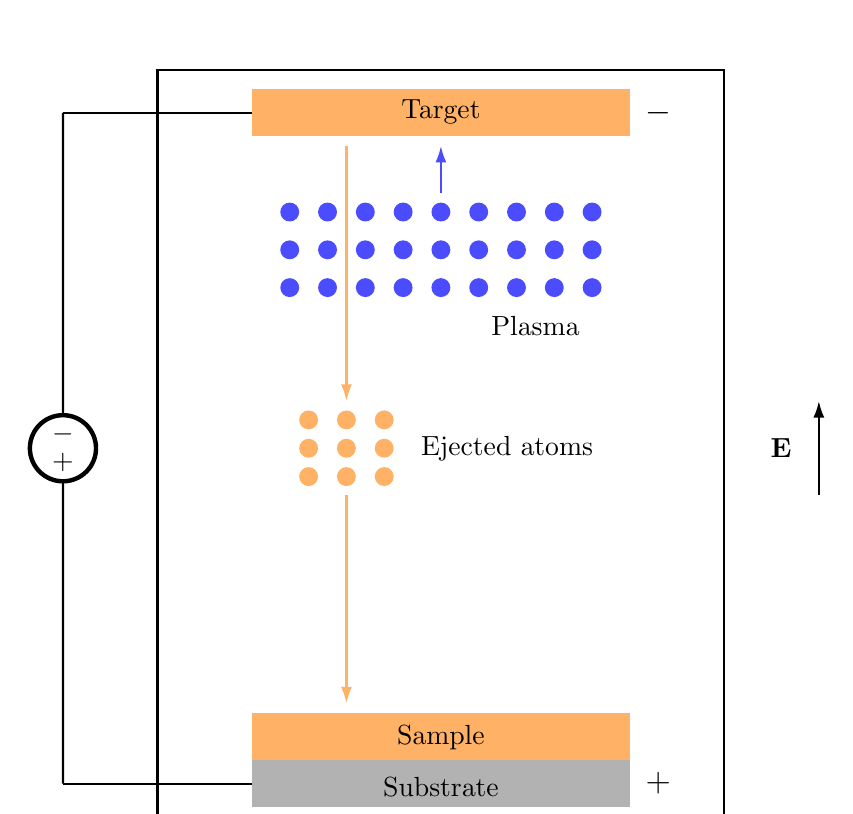
\begin{tikzpicture}[scale=1.2, thick]
		
		% Chamber rectangle
		\draw (0,0) rectangle (6,8);
		
		% Target (top)
		\fill[orange!60] (1,7.3) rectangle (5,7.8);
		\node at (3,7.8) [below] {Target};
		\node at (5.3,7.55) {\large$-$};
		
		% Substrate (bottom)
		\fill[gray!60] (1,0.2) rectangle (5,0.7);
		\node at (3,0.2) [above] {Substrate};
		\node at (5.3,0.45) {\large$+$};
		
		% Sample
		\fill[orange!60] (1,0.7) rectangle (5,1.2);
		\node at (3,0.7) [above] {Sample};
		
		% Plasma (some circles in the middle)
		\foreach \x in {1.4,1.8,2.2,2.6,3,3.4,3.8,4.2,4.6}
		\fill[blue!70] (\x,6.5) circle (0.1);
		
		\foreach \x in {1.4,1.8,2.2,2.6,3,3.4,3.8,4.2,4.6}
		\fill[blue!70] (\x,6.1) circle (0.1);
		
		\foreach \x in {1.4,1.8,2.2,2.6,3,3.4,3.8,4.2,4.6}
		\fill[blue!70] (\x,5.7) circle (0.1);
		
		\node at (4,5.3) {Plasma};
		
		\draw[-{Latex[length=6pt,width=4pt]}, blue!70] (3, 6.7) -- (3,7.2);
		
		% Ejected atoms
		\foreach \x in {1.6,2,2.4}
		\fill[orange!60] (\x,4.3) circle (0.1);
		
		\foreach \x in {1.6,2,2.4}
		\fill[orange!60] (\x,4) circle (0.1);
		
		\foreach \x in {1.6,2,2.4}
		\fill[orange!60] (\x,3.7) circle (0.1);
		
		\node at (3.7,4) {Ejected atoms};
		
		\draw[-{Latex[length=6pt,width=4pt]}, orange!60] (2,7.2) -- (2,4.5);
		
		\draw[-{Latex[length=6pt,width=4pt]}, orange!60] (2,3.5) -- (2,1.3);
		
		% DC voltage source
		\draw (1,0.45) -- (-1,0.45);
		\draw (-1,0.45) to[american voltage source] (-1,7.55);
		\draw (-1,7.55) -- (1,7.55);
		
		% Electric field
		\draw[-{Latex[length=6pt,width=4pt]}] (7,3.5) -- (7,4.5);
		\node at (6.6,4) {$\mathbf{E}$};
		
	\end{tikzpicture}
	\caption{Schematic illustration of a sputtering device.}
	
	\label{Sputtering}
\end{figure}
 
The structures investigated in this work are listed in the following table. Tables \ref{Samples_dimensions_1} shows the thicnkesses of the layers of the samples used in the control sample, bilayer and microwave power experiments (these experiments used a single sample). Table \ref{Samples_dimensions_2} and table \ref{Samples_dimensions_3} show the thicknesses of the layers for the copper thickness and permalloy thickness experiments respectively. 

\begin{table}[H]
	\centering
	\begin{tabular}{c c c}
		\hline
		\rule{0pt}{2.5ex}\rule[-1.2ex]{0pt}{0pt}  % <-- spazio extra sopra e sotto
		Sample & Nb thickness (nm) & Py thickness (nm) \\
		\hline
		Control Sample & $80 \pm2.4$ & 0            \\
		Bilayer & $80 \pm2.4$ & $2 \pm 0.06$  \\                    
		Microwave Power & $80 \pm2.4$ & $5 \pm 0.15$  \\
		\hline                   
	\end{tabular}
	\caption{List of samples used in this study.}
	\label{Samples_dimensions_1}
	\end{table}
	
\begin{table}[H]
	\centering
	\begin{tabular}{c c c c}
		\hline
		\rule{0pt}{2.5ex}\rule[-1.2ex]{0pt}{0pt}  % <-- spazio extra sopra e sotto
		Sample & Nb thickness (nm) & Cu thickness (nm) & Py thickness (nm) \\
		\hline
		S$_0$ & $80 \pm2.4$ & 0            & $20 \pm 0.6$ \\
		S$_1$ & $80 \pm2.4$ & $2 \pm 0.06$ & $20 \pm 0.6$ \\                    
		S$_2$ & $80 \pm2.4$ & $5 \pm 0.15$ & $20 \pm 0.6$ \\                   
		S$_3$ & $80 \pm2.4$ & $10 \pm 0.3$ & $20 \pm 0.6$ \\                     
		S$_4$ & $80 \pm2.4$ & $20 \pm 0.6$ & $20 \pm 0.6$ \\                      
		S$_5$ & $80 \pm2.4$ & $50 \pm 1.5$ & $20 \pm 0.6$ \\                 
		S$_6$ & $80 \pm2.4$ & $100 \pm 3$  & $20 \pm 0.6$ \\            
		S$_7$ & $80 \pm2.4$ & $200 \pm 6$  & $20 \pm 0.6$ \\
		\hline
	\end{tabular}
	\caption{List of samples used in this study.}
	\label{Samples_dimensions_2}
\end{table}

The samples were characterized using atomic force microscopy (AFM), which is a type of scanning probe microscopy that maps the surface topography of a sample with nanometer resolution by mechanically probing it with a sharp tip. The core of an AFM consists of a cantilever with a sharp tip that interacts with the sample surface through intermolecular forces between the atoms at the tip and the sample that cause the cantilever to deflect. This deflection is measured by a laser beam reflected from the cantilever onto a position-sensitive photodiode. A feedback circuit maintains a constant interaction between the tip and the surface by adjusting the vertical position of the scanner. The height adjustments required to maintain the set interaction force are recorded to reconstruct the surface topography. This allowed to calculate the 3\% errors on the thickness of the layers. Figure \ref{AFM} shows the general scheme of a setup used for AFM measurements.

\begin{figure}[H]
	\centering
	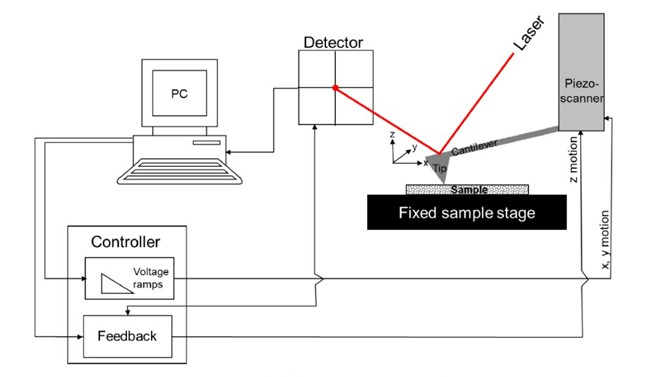
\includegraphics[width=0.75\linewidth]{Immagini/Experimental_setup_images/AFM_scheme.jpg}
	\caption{Schematic representation of an AFM setup.}
	\label{AFM}
\end{figure}


\section{Experimental Setup}
The samples are mounted using vacuum grease onto a coplanar waveguide (CPW) and placed into a cryostat. A CPW is a planar transmission line structure consisting of a central conducting strip separated by narrow gaps from two ground planes, all defined on the same surface of a dielectric substrate. The signal propagates along the central conductor, while the two adjacent ground planes provide a return path. The sample is placed upside down (with the upper superconducting layer of figure \ref{Samples} in contact with the CPW) because the magnetic field generated by the current in the CPW is stronger in the small region close to the surface and, due to the substrate being much thicker then the other layers, placing it the other way would make the magnetic field in the Py layer too weak to be measured. The external magnetic field and cryogenic environment are provided by the Oxford Instruments Teslatron cryostat, which contains a superconducting vector magnet with 6 T in the z-direction, 2 T in the x- and y-directions, and a base temperature of 1.5K. The sample is mounted on a sample probe, where the thickness lies in the x-direction, and is designed so that the sample is positioned between the superconducting coils to maximise the uniformity of the field. Steel coaxial cables run down the length of the sample probe and act as microwave transmission lines to the CPW. Connected to the top of the cryostat, there are copper coaxial cables. The first copper cable acts as the input and is connected to a microwave generator, which drives the AC field that excites the sample. The second cable is connected to a microwave detector, which is directly connected to a lock-in amplifier. Figure \ref{Probe_setup} shows a schematic diagram of the cryostat and probe assembly while figure \ref{Probe_picture} shows an actual picture of the probe and sample.

\begin{figure}[H]
	\centering
	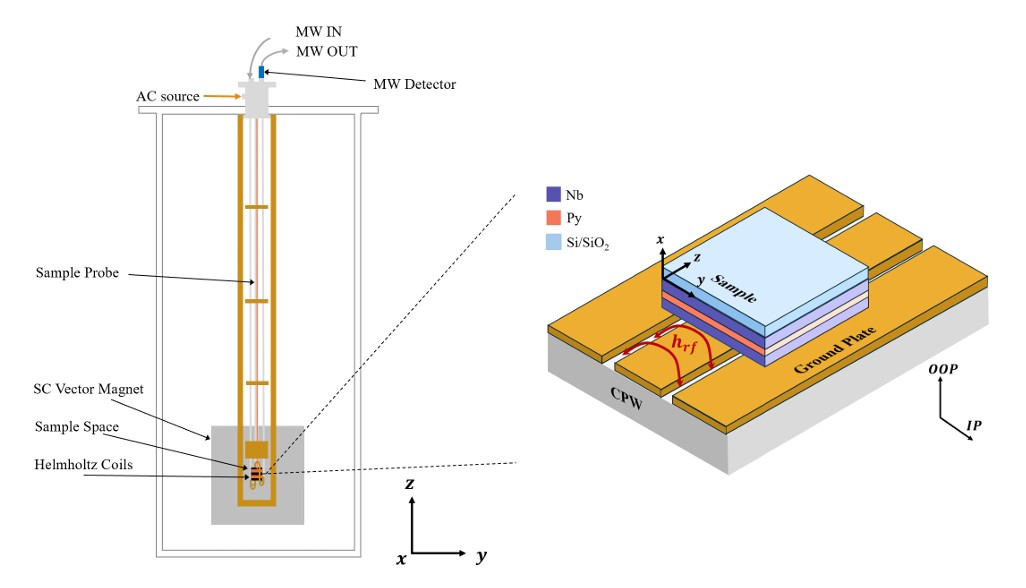
\includegraphics[width=\linewidth]{Immagini/Experimental_setup_images/Probe_setup.jpg}
	\caption{Schematic diagram of the cryostat and probe assembly.}
	\label{Probe_setup}
\end{figure}

\begin{figure}[H]
	\centering
	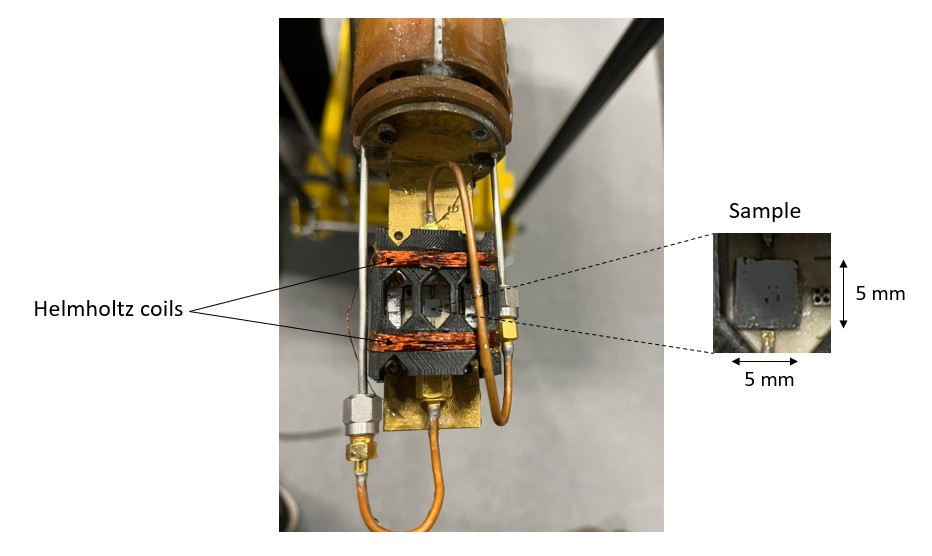
\includegraphics[width=\linewidth]{Immagini/Experimental_setup_images/Probe_picture_3.jpg}
	\caption{Picture of the sample and probe assembly.}
	\label{Probe_picture}
\end{figure}

Figure \ref{fig:FMR_setup} shows a schematic of the complete setup used to conduct the FMR measurements. A signal is sent from a microwave source to the CPW through a coaxial cable, the current flowing in the CPW creates an oscillating magnetic field at the same microwave frequency as the input signal. According to Biot–Savart law, this field lies along the $y$ axis and is approximately uniform across the sample. Together with the static magnetic field produced by the superconducting coil of the cryostat, which is constant in time, approximately uniform along the sample, and oriented along the $z$ axis, this oscillating field can, in principle, induce ferromagnetic resonance. However, this effect is difficult to detect directly due to noise; therefore, a universal source, a pair of Helmholtz coils, and a lock-in amplifier are introduced to improve signal detection. Part of the energy carried by the signal is absorbed by the sample through FMR. The resulting transmitted signal is then sent to a diode, a composite component that converts the AC signal into a DC signal with an amplitude proportional to the average power of the input signal. The universal source sends a signal at 321 Hz to the two Hemholtz coils, generating a magnetic field whose frequency is much lower than the MW frequency of the input signal. This field can therefore be considered constant in time and added to the DC magnetic field generated by the electromagnet, the lock-in amplifier then registers the variation in the diode voltage $\delta V_{diode}$ caused by a small variation $\delta H_{DC}$ of the DC magnetic fields and returns a signal proportional to the ratio $\frac{\delta V_{diode}}{\delta H_{DC}}$ which is approximately equal to the derivative of $V_{diode}$ with respect to $H_{DC}$. 

\begin{figure}[H]
	\centering
	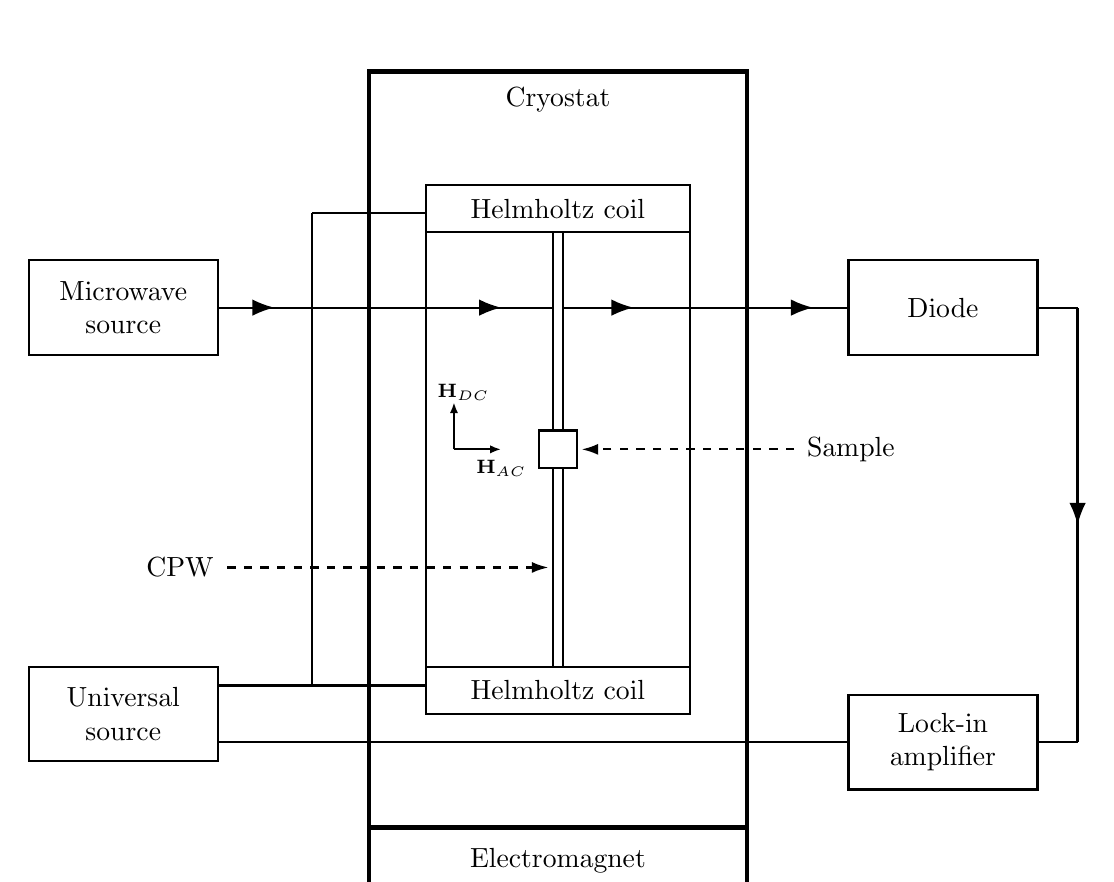
\begin{tikzpicture}[scale=1.2, thick]
		
		% CPW
		\draw (-1.4,-2.3) rectangle (1.4,2.3);
		
		\draw (-0.2,-0.2) rectangle (0.2,0.2); %Sample
		
		\draw (-0.05,-2.3) to (-0.05,-0.2);
		\draw (0.05,-2.3) to (0.05,-0.2);
		\draw (-0.05,2.3) to (-0.05,0.2);
		\draw (0.05,2.3) to (0.05,0.2);
		
		\draw[dashed,-{Latex[length=6pt,width=4pt]}] (-3.5,-1.25) -- (-0.1,-1.25);
		\node[align=center] at (-4,-1.25) {CPW};
		
		\draw (-1.4, -2.3) rectangle (1.4,-2.8); %Helmholtz coil
		\draw (-1.4, 2.3) rectangle (1.4,2.8); %Helmholtz coil
		%\draw[dashed,-{Latex[length=6pt,width=4pt]}] (1.95,-1) -- (0.8,-1.6);
		\node[align=center] at (0,-2.55) {Helmholtz coil};
		%\draw[dashed,-{Latex[length=6pt,width=4pt]}] (1.95, 2.2) -- (0.8,1.6);
		\node[align=center] at (0,2.55) {Helmholtz coil};
		
		\draw[dashed,-{Latex[length=6pt,width=4pt]}] (2.5,0) -- (0.25,0); 
		\node[align=center] at (3.1,0) {Sample};
		
		%Magnetic fields
		\draw[-{Latex[length=4pt,width=3pt]}] (-1.1,0) -- (-1.1,0.5); 
		\node[align=center] at (-1,0.6) {\scriptsize $\mathbf{H}_{DC}$};
		\draw[-{Latex[length=4pt,width=3pt]}] (-1.1,0) -- (-0.6,0); 
		\node[align=center] at (-0.6,-0.2) {\scriptsize $\mathbf{H}_{AC}$};
		
		% MW source
		\draw (-5.6, 1) rectangle (-3.6,2);
		\draw (-3.6, 1.5) -- (-0.05,1.5);
		\draw[-{Latex[length=8pt,width=6pt]}] (-3.5,1.5) -- (-3,1.5);
		\draw[-{Latex[length=8pt,width=6pt]}] (-1.2,1.5) -- (-0.6,1.5);
		\node[align=center] at (-4.6,1.5) {Microwave \\ source};
		
		%Universal source
		\draw (-5.6, -2.3) rectangle (-3.6,-3.3);
		\draw (-3.6, -2.5) to (-1.4,-2.5);
		\draw (-3.6, -3.1) to (3.075,-3.1);
		\draw (-2.6, -2.5) to (-2.6,2.5);
		\draw (-2.6, 2.5) to (-1.4,2.5);
		\node[align=center] at (-4.6,-2.8) {Universal \\ source};
		
		%Diode
		\draw (0.05, 1.5) to (3.075,1.5);
		\draw (3.075, 1) rectangle (5.075,2);
		\draw (5.075, 1.5) to (5.5,1.5);
		\draw[-{Latex[length=8pt,width=6pt]}] (2,1.5) -- (2.7,1.5);
		\draw[-{Latex[length=8pt,width=6pt]}] (0.2,1.5) -- (0.8,1.5);
		\node at (4.075,1.5) {Diode};
		
		%Lock-in amplifier
		\draw (3.075, -2.6) rectangle (5.075,-3.6);
		\draw (5.075, -3.1) to (5.5, -3.1);
		\draw (5.5,-3.1) to (5.5,1.5);
		\draw[-{Latex[length=8pt,width=6pt]}] (5.5,0) -- (5.5,-0.8);
		\node[align=center] at (4.075,-3.1) {Lock-in \\ amplifier};
		
		%Cryostat
		\draw[ultra thick] (-2,-4) rectangle (2,4);
		\draw[ultra thick] (-2,-4) rectangle (2,-4.7);
		\node[align=center] at (0,3.7) {Cryostat};
		\node[align=center] at (0,-4.35) {Electromagnet};
		
	\end{tikzpicture}
	\caption{Schematic illustration of the setup used in the experiment.}
	
	\label{fig:FMR_setup}
\end{figure} 

\section{FMR Measurements}
Ferromagnetic resonance can be conducted by either sweeping frequency or magnetic field. In this case, the FMR absorption spectrum is detected by changing the external magnetic field at fixed frequencies to find the resonance field. As explained in the previous section, the resulting data is in the form of the derivative of the Lorentzian, which is analysed using the symmetric and antisymmetric lorentzian functions with respect to $H_{res}$. Another effect that is observed is that the data present a linear noise that is added to the lorentzian derivative function, therefore the profile of the data is expected to look like figure \ref{Lorentzian_signal}. The origin of the linear noise is still not known. A possible explanation for the linear noise is an impedance mismatch in the connections between the microwve generator and the CPW and between the CPW and the diode.
\begin{figure}[H]
	\centering
	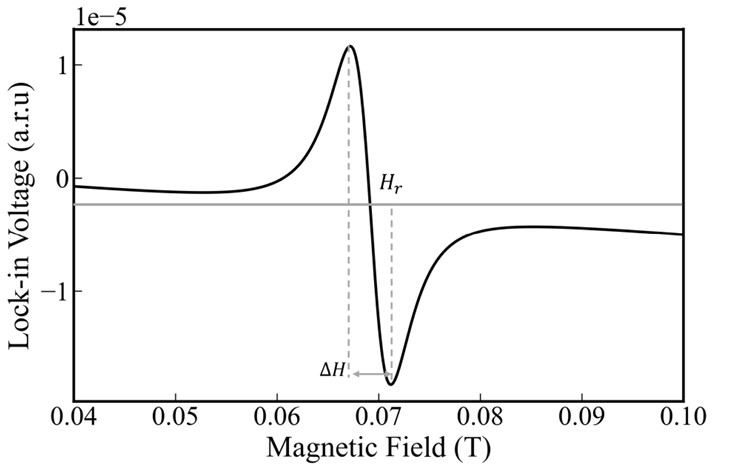
\includegraphics[width=0.8\linewidth]{Immagini/Experimental_setup_images/Lorentzian_signal.jpg}
	\caption{Expected behaviour of the signal}
	\label{Lorentzian_signal}
\end{figure}

From this, the resonant field and linewidths can be extracted from each scan at each frequency and temperature by doing a fit on the data with a lorentzian derivative combined with a linear background. The values of resonant field and resonant frequency can be analyzed to form the Kittel relationship, allowing for exploration of changes in the resonant frequency-resonant field relationship. Apart from the bilayer sample, which is expected to follow the standard Kittel equation \ref{eq:Kittel}, the other samples are expected to exhibit anisotropy consistent with the modified Kittel equation \ref{eq:Kittel_modified}.
\chapter{Data analysis and Results}

\section{Previous Literature (?)}
The first step of the investigation was to reproduce the results reported in the literature \cite{Magnetization}. Specifically, it is known that introducing two superconducting thin film layers around a ferromagnetic thin film generates a shift in the resonant field $H_{res}$, which therefore follows the modified Kittel equation \ref{eq:Kittel_modified} instead of the standard one \ref{eq:Kittel}. This shift appears only below a certain critical temperature, and both superconducting layers are required for the effect to occur. The first two conditions were verified using the control sample, while the last one was confirmed with the bilayer sample.

\subsection{Control Sample}
For different values of the temperature $T$ and frequency $f$, the lock-in voltage was measured as a function of the applied DC magnetic field. All measurements were performed from 10 K down to 1.5 K over a frequency range of 6 to 15 GHz, using field-modulation FMR. As explained in the previous chapter, the signal detected by the lock-in amplifier is proportional to the derivative with respect to the magnetic field $H$ of the signal from the CPW. Therefore, the data were fitted using the following equation:
\begin{align}
	V = S \dfrac{\Delta H^2 (H-H_{res})}{(\Delta H^2 + (H-H_{res})^2)^2} + A \dfrac{\Delta H (H-H_{res})^2 - \Delta H^3}{(\Delta H (H-H_{res})^2)^2} + aH+d
\end{align}
From this expression, the resonant field can be identified as the point where the function, excluding the linear background, crosses zero. Figure \ref{fig:raw_plot_example} shows a representative plot of the measured data.

\begin{figure}[H]
	\centering
	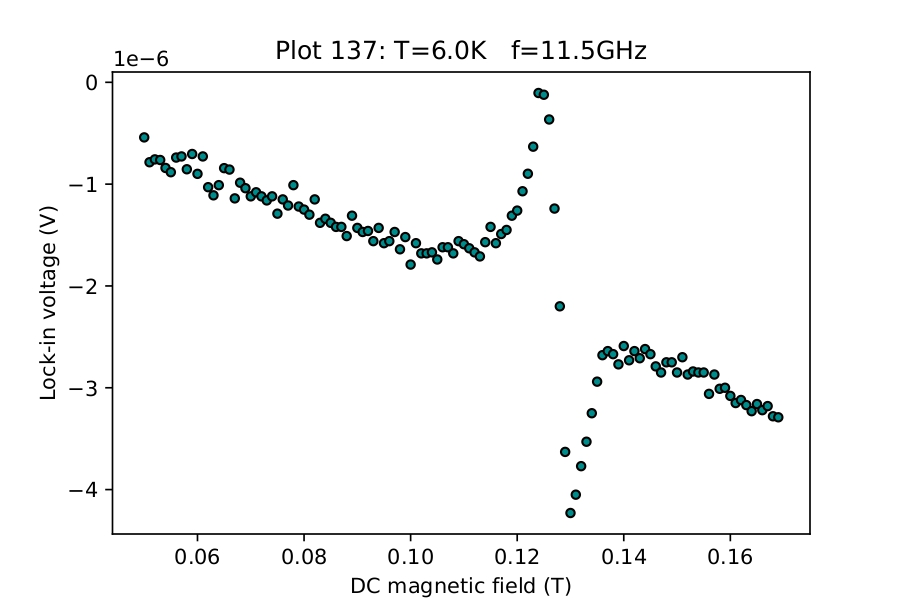
\includegraphics[width=\linewidth]{Immagini/Data_images/Control_sample_images/raw_plots_pages-to-jpg-0137.jpg}
	\caption{Experimental data for the DC magnetic field and lock-in voltage.}
	\label{fig:raw_plot_example}
\end{figure}

As expected, the plot follows the qualitative behaviour shown in Figure \ref{Lorentzian_signal}. To fit the data, the linear background was first removed. This was done by performing a linear fit over the entire dataset. Because the number of points around the resonant field was much smaller than the number of points in the linear regime, this approach provided a reliable estimate of the parameters $a$ and $d$. Figure \ref{fig:linear_plot_example} shows the data from Figure \ref{fig:raw_plot_example} together with their fitted linear component.
\begin{figure}[H]
	\centering
	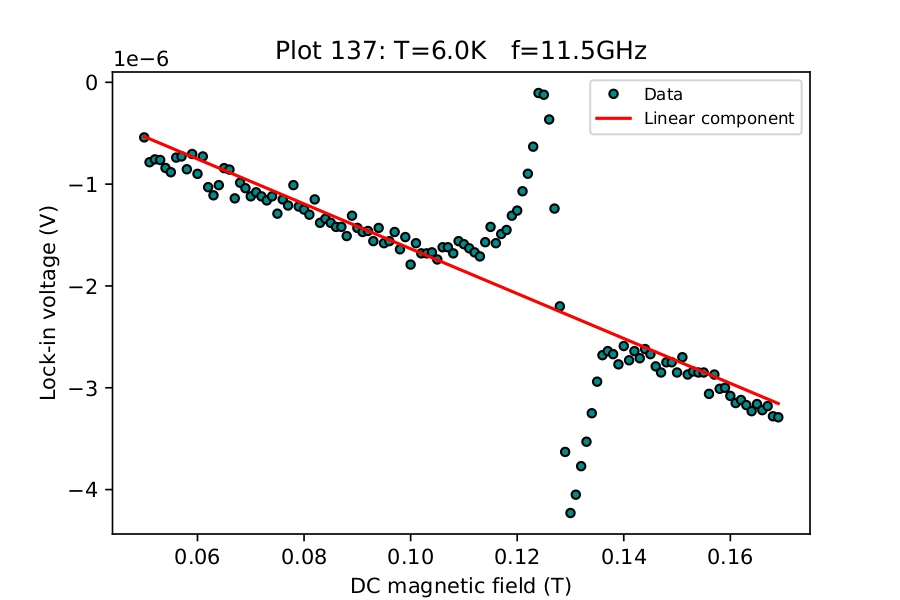
\includegraphics[width=\linewidth]{Immagini/Data_images/Control_sample_images/all_linear_fits_page-0137.jpg}
	\caption{Linear component extrapolated from a fit on the entire dataset.}
	\label{fig:linear_plot_example}
\end{figure}

The linear component was then subtracted from the data and a four parameter fit was made on the resulting dataset. The initial guess values for the parameters $H_{res}$, $\Delta H$, $S$, $A$ were calculated using the following formulas:

\begin{empheq}{align}
	&H^{res}_{guess} = \dfrac{H_{max}+H_{min}}{2} \label{eq:guess_Hres} \\
	&\Delta H_{guess} = 0.1(H_{max}-H_{min}) \label{eq:guess_DeltaH} \\
	&S_{guess} = 0.7(V_{max}-V_{min}) \label{eq:guess_S} \\
	&A_{guess} = 0.3(V_{max}-V_{min}) \label{eq:guess_A}
\end{empheq}

Where $V_{max}$ and $V_{min}$ are the maximum and minimum value of the lock-in voltage in the data, while $H_{max}$ and $H_{min}$ are the corresponding values of the DC magnetic field. Figure \ref{fig:guesses_example} shows the same dataset together with the initial guess curve, figure \ref{fig:fits_example} displays the final fitted curve.

\begin{figure}[H]
	\centering
	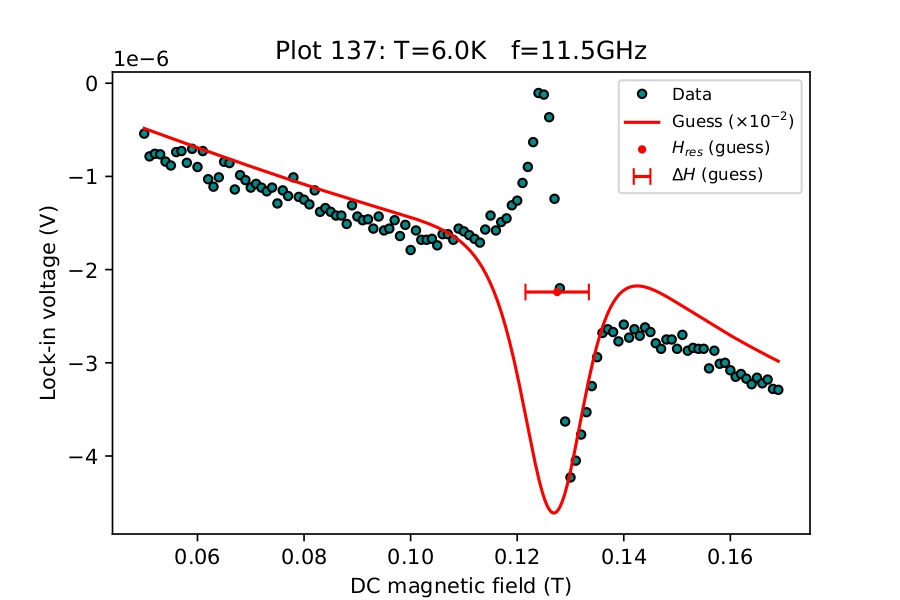
\includegraphics[width=1\linewidth]{Immagini/Data_images/Control_sample_images/guesses_page-0137.jpg}
	\caption{Guess curve obtained from equations \ref{eq:guess_Hres} - \ref{eq:guess_A}.}
	\label{fig:guesses_example}
\end{figure}

\begin{figure}[H]
	\centering
	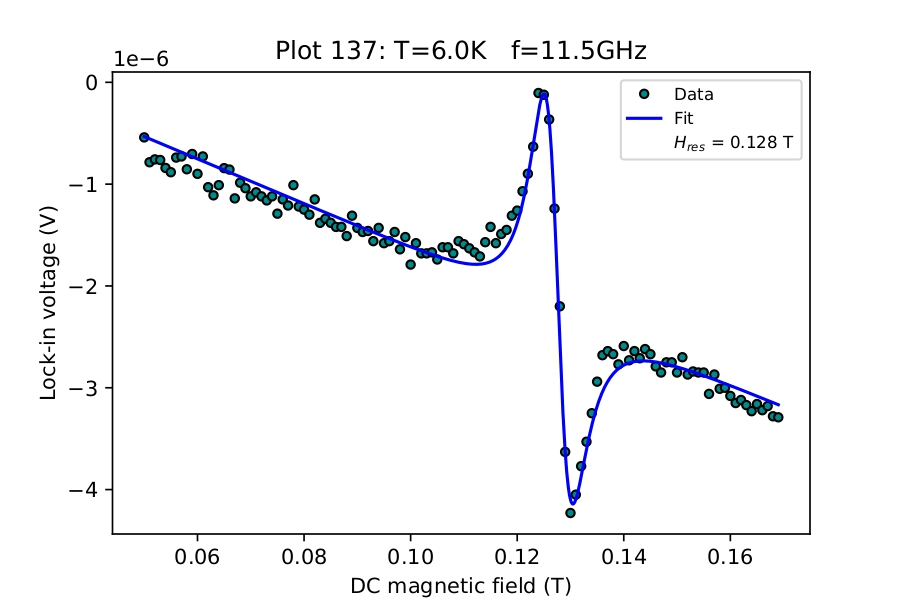
\includegraphics[width=\linewidth]{Immagini/Data_images/Control_sample_images/fits_page-0137.jpg}
	\caption{Fit curve obtained from the previous guess.}
	\label{fig:fits_example}
\end{figure}

For each temperature the values of resonant frequency and field were fitted with the modified Kittel's equation
\begin{align}
	f_{res} = \dfrac{\gamma}{2 \pi} \sqrt{(H_{res}+H_a)(H_{res}+H_a+M_{eff})}
\end{align}
to find the anisotrpy field $H_a$. Figure \ref{fig:Kittel_fit} shows an example of a dataset together with its fitted curve.

\begin{figure}[H]
	\centering
	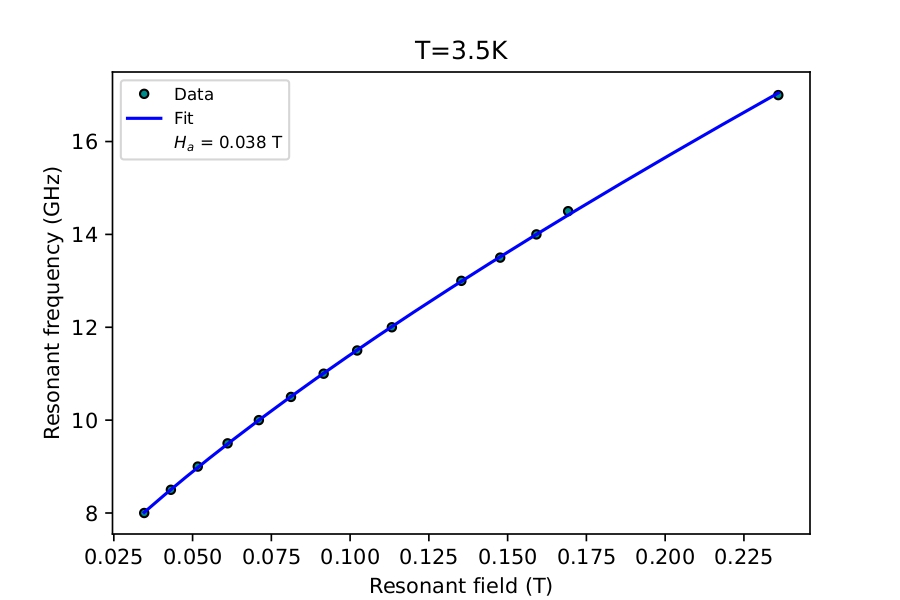
\includegraphics[width=\linewidth]{Immagini/Data_images/Control_sample_images/Kittel_fits_page-0005.jpg}
	\caption{Experimental data for resonant field and resonant frequency at $T=3.5K$.}
	\label{fig:Kittel_fit}
\end{figure}

\begin{figure}[H]
	\centering
	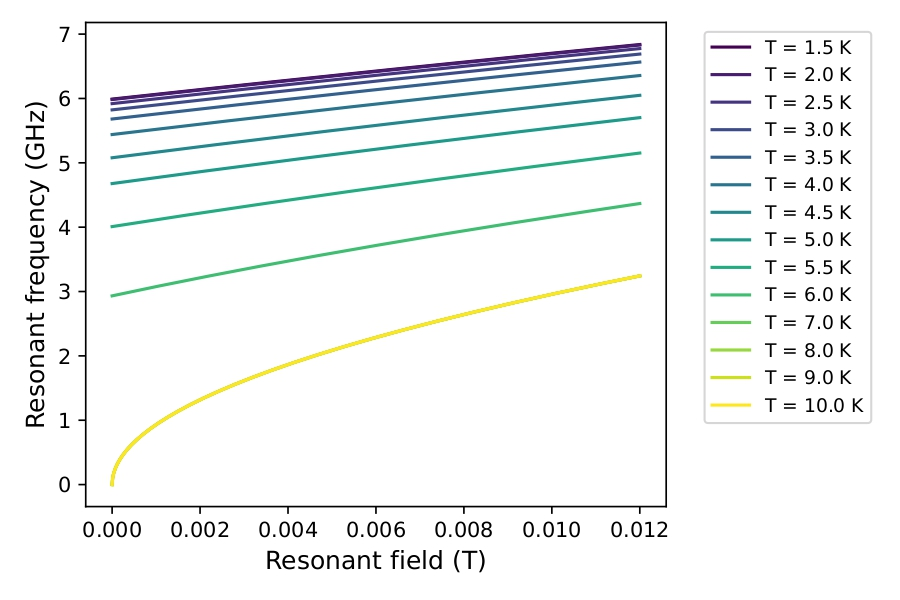
\includegraphics[width=\linewidth]{Immagini/Data_images/Control_sample_images/Kittel_in_one_page-0001 (1).jpg}
	\caption{Fitted curves of the Kittel equation for different temperatuers.}
	\label{fig:Kittel_in_one}
\end{figure}
As expected, the curves below the critical temperature coincide, confirming that no change in the anisotropy occurs in this regime. In contrast, the curves above the critical temperature display an offset that increases as the temperature decreases. Finally, the values of the anisotropy field $H_a$ were plotted as a function of the temperature $T$ to verify that the shift in $H_{res}$ appears only below the critical temperature $T_c$. The resulting plot is shown in Figure \ref{H_a_vs_T}.

\begin{figure}[H]
	\centering
	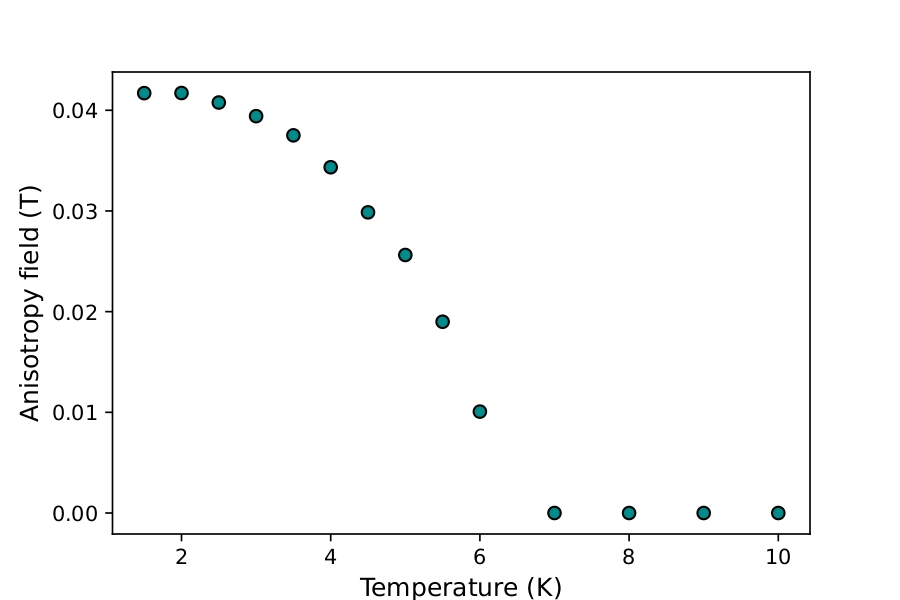
\includegraphics[width=\linewidth]{Immagini/Data_images/Control_sample_images/Ha_vs_T_page-0001.jpg}
	\caption{Anisotropy field as a function of temperature.}
	\label{H_a_vs_T}
\end{figure}

As expected, $H_a$ has a constant value of zero below $T_c$. The observed critical temperature is lower than the theoretical critical temperature of niobium (9 K), this can be attributed to a proximity effect. This plot confirms that superconductivity is a continuous phase transition, as no discontinuity is observed in $H_a$, and that the anisotropy field can be used as an order parameter for the trilayer system. 

The data for the anisotrpy field with $H_a > 0 $ were then fitted with the power law \ref{eq:power_law} and the following values for the critical temperature $T_C$ and for the exponent $p$ were obtained
\begin{empheq}{align}
	& T_c = 6.5 \pm 0.027 \, \text{K} \\
	& p = 3.489 \pm 0.095  
\end{empheq}
Figure \ref{fig:Ha_fit} shows the comparison between the data and the fit curve
\begin{figure}[H]
	\centering
	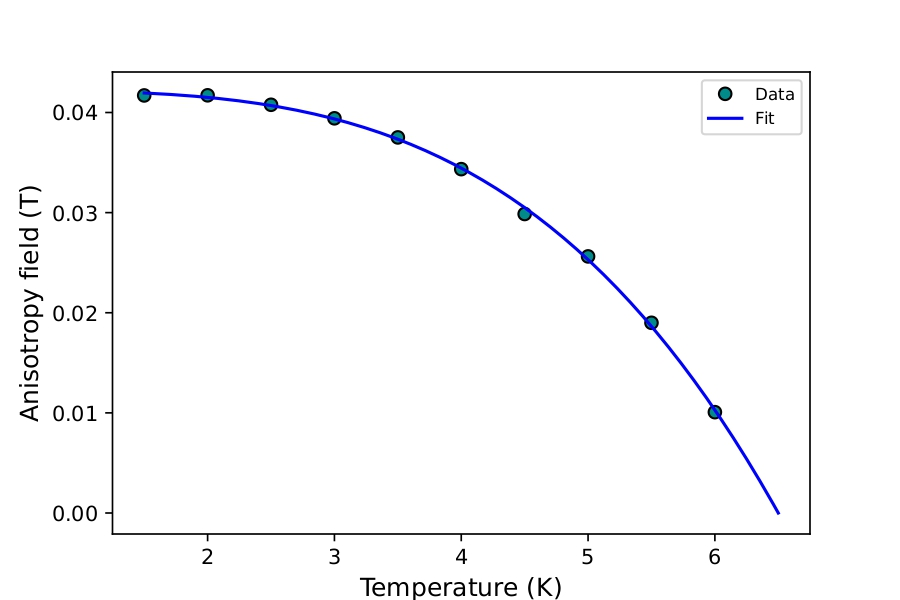
\includegraphics[width=\linewidth]{Immagini/Data_images/Control_sample_images/Ha_fit_page-0001.jpg}
	\caption{Values of the anisotropy field with the fit curve obtained from the power law below $T_c$.}
	\label{fig:Ha_fit}
\end{figure}

\newpage

\subsection{Bilayer}
The same procedure used for the control sample was used for the bilayer sample. Figure \ref{fig:Ha_vs_T_bilayer} shows the values of the anisotropy field for different temperatures both above and below the critical temperature.
\begin{figure}[H]
	\centering
	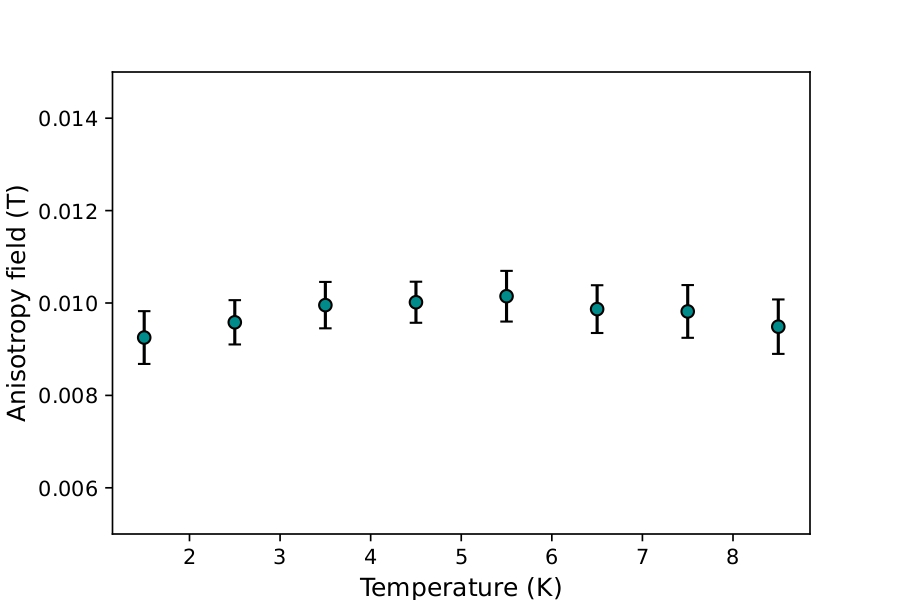
\includegraphics[width=\linewidth]{Immagini/Data_images/Bilayer_images/Bilayer_Ha_vs_T_page-0001.jpg}
	\caption{Anisotrpy field for different temperatures in the asymmetric sample.}
	\label{fig:Ha_vs_T_bilayer}
\end{figure}
In this case there, no change in the anisotropy field is observed below the critical temperature within the experimental errors. This indicates that both superconducting layers are required in order to produce the change in anisotropy. Moreover, the anisotropy field remains greater than zero even below the critical temperature, this is due to shape anisotropy and impurities in the sample.

\newpage

\section{New Experiments (?)}
The next step of the investigation was to test the theory presented in \cite{Russian} by conducting FMR measurements on a thin film multilayer containing two additional metallic (Cu) layers, as well as on a trilayer at different microwave power levels. The aim is to determine whether the effect exhibits any dependence on the microwave power, which is expected for a dynamical mechanism such as the one proposed in \cite{Russian}, and whether the introduction of metallic layers (through which electric currents can flow) leads to any modification of the observed behavior.

\subsection{Copper Thickness}
The same procedure described in the previous section was used to extract the values of the resonant field for samples with additional copper layers of thicknesses ranging from 2 nm to 100 nm. For the sample with a 200 nm Cu layer, it was not possible to obtain reliable data because, in this case, the ferromagnetic layer was too far from the CPW and the resulting microwave magnetic field was too weak to be detected. The anisotropy field values for the different samples below the critical temperature are shown in figure \ref{fig:Ha_vs_Cu}.
\begin{figure}[H]
	\centering
	\hspace*{-0.7cm} % sposta verso sinistra
	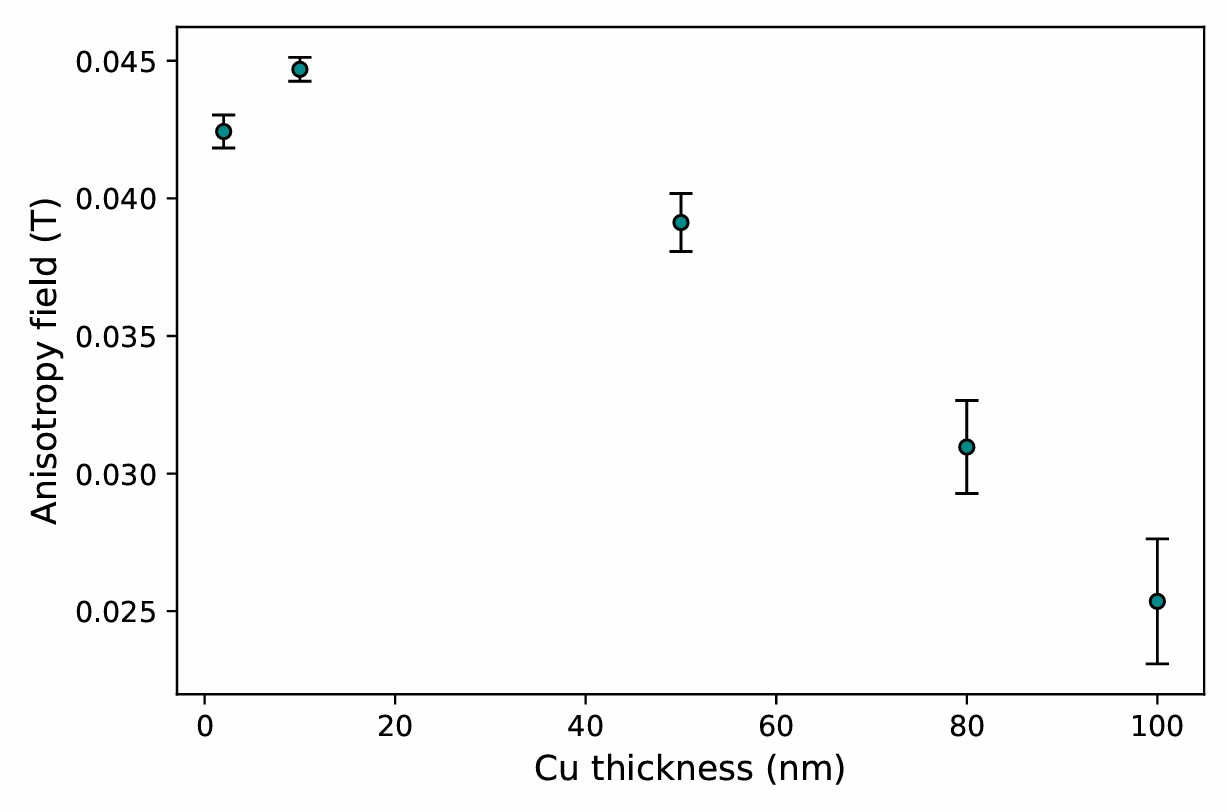
\includegraphics[width=0.9\linewidth]{Immagini/Data_images/Ha_vs_Cu.jpg}
	\caption{Anisotropy field at $T=2.0K$ for different thicknesses of the Cu layers.}
	\label{fig:Ha_vs_Cu}
\end{figure}
Although the plot does not contain enough data points to draw a definitive conclusion about the behavior of the anisotropy field as a function of the copper thickness, it clearly shows that the effect does not disappear upon introducing a conducting layer, as it does when an insulating layer is inserted. This observation suggests that the effect is linked to currents flowing through the entire system.

\subsection{Microwave Power}
The values of the resonant field extracted from the Kittel fits at different microwave powers are shown in figure \ref{fig:Hres_vs_MWPower}.
\begin{figure}[H]
	\centering
	\hspace*{-0.5cm} % sposta verso sinistra
	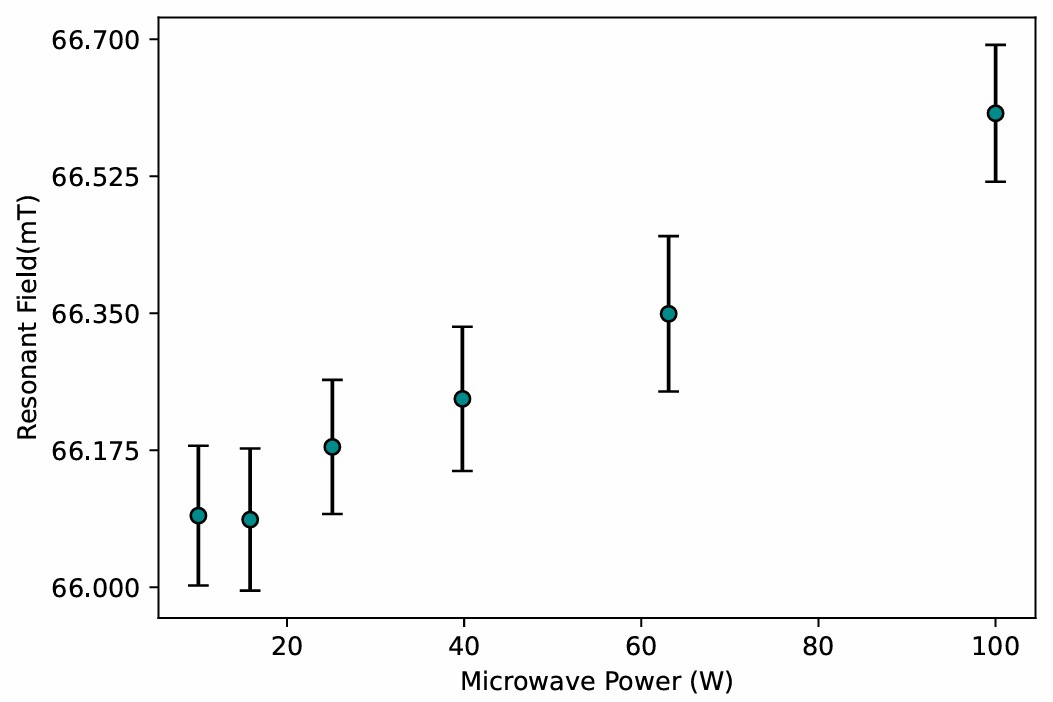
\includegraphics[width=0.9\linewidth]{Immagini/Data_images/Hres_vs_MWpower.jpg}
	\caption{Anisotropy field at $T=2.0K$ for different values of the microwave power.}
	\label{fig:Hres_vs_MWPower}
\end{figure}
A variation in the resonant field is observed; however, this is most likely due to heating of the system. The microwave signal induces eddy currents in the trilayer, which raise its temperature and thereby reduce the anisotropy field, resulting in a small shift of the resonant field. It can therefore be concluded that the effect is independent of the microwave power.

\section{Results}
This thesis presented an experimental investigation of the superconductivity-induced shift in the ferromagnetic resonant field observed in superconductor–ferromagnet–superconductor (S/F/S) trilayers. .

The first part of the study confirmed the core results reported in earlier works: when the ferromagnetic layer is coupled with two superconducting layers, the resonant field extracted from ferromagnetic resonance (FMR) measurements deviates from the standard Kittel relation \ref{eq:Kittel} and instead follows a modified form \ref{eq:Kittel_modified} containing an additional anisotropy field. This additional term appears only below the superconducting critical temperature and increases as the temperature decreases, demonstrating a clear connection between the effect and the superconducting phase. Furthermore, the bilayer measurements showed no detectable change in the resonant field across the superconducting transition, confirming that both superconducting layers are required for the effect to occur. These outcomes reproduce the essential features found in the literature (\cite{Magnetization}, \cite{First_Evidence_1}, \cite{First_Evidence_2}).

In the second part of the work, other experiments were performed to probe the origin of the additional anisotropy field. Measurements on multilayers containing copper spacers of varying thicknesses showed that the effect persists even when metallic layers are inserted between the superconducting and ferromagnetic layers. In contrast, previous studies have shown that inserting an insulating layer suppresses the effect entirely. This comparison suggests that the phenomenon is associated with electrical currents flowing through the multilayer system, rather than arising from a purely local interfacial mechanism.

Additional measurements were carried out at different microwave power levels to determine whether the shift might originate from a dynamical mechanism, as suggested in \cite{Russian}. The experimental results showed small variations in the resonant field with microwave power that are consistent with thermal effects due to microwave-induced heating. No significant dependence on the microwave power was observed, indicating that the effect does not originate from the dynamical effect within the accessible power range.

%\printbibliography
\printbibliography[heading=bibintoc,title={Bibliography}]

\chapter*{Aknowlesgements/Ringraziamenti}
%\addcontentsline{toc}{chapter}{Ringraziamenti}

\end{document}